\documentclass[thesis-en.tex]{subfiles}

\graphicspath{{images/results/}}

\newcommand{\figh}{0.2}
\newcommand{\sfigw}{0.325}

\newcommand{\resplot}[3]{
\begin{figure}[hp]
  \begin{subfigure}{\sfigw\linewidth}
    \centering
    \includegraphics[width=\linewidth,height=\linewidth]{reservation_#1_#2_mean.pdf} 
    \caption{Mean (logarithmic)} 
    \label{fig:reservation_#1_#2_mean} 
  \end{subfigure}
  \hfill
  \begin{subfigure}{\sfigw\linewidth}
    \centering
    \includegraphics[width=\linewidth,height=\linewidth]{reservation_#1_#2_boxen.pdf}
    \caption{Quantiles (logarithmic)}
    \label{fig:reservation_#1_#2_boxen}
  \end{subfigure}
  \hfill
  \begin{subfigure}{\sfigw\linewidth}
    \centering
    \includegraphics[width=\linewidth,height=\linewidth]{reservation_#1_#2_dist.pdf}
    \caption{Tail distribution} 
    \label{fig:reservation_#1_#2_dist} 
  \end{subfigure}
  \caption{#3}
  \label{fig:reservation_#1_#2} 
\end{figure}
}

\newcommand{\loadplot}[3]{
\begin{figure}[p] 
  \begin{subfigure}{0.5\linewidth}
    \centering
    \includegraphics[width=\linewidth,height=\figh\textheight]{reservation_#1_#2_fcfs.pdf} 
    \caption{fcfs} 
    \label{fig:reservation_#1_#2_fcfs} 
  \end{subfigure}
  \hfill
  \begin{subfigure}{0.5\linewidth}
    \centering
    \includegraphics[width=\linewidth,height=\figh\textheight]{reservation_#1_#2_future.pdf} 
    \caption{no-future-1} 
    \label{fig:reservation_#1_#2_future}
  \end{subfigure} 
  \begin{subfigure}{0.5\linewidth}
    \centering
    \includegraphics[width=\linewidth,height=\figh\textheight]{reservation_#1_#2_backfill.pdf} 
    \caption{backfill-1} 
    \label{fig:reservation_#1_#2_backfill} 
  \end{subfigure}
  \hfill
  \begin{subfigure}{0.5\linewidth}
    \centering
    \includegraphics[width=\linewidth,height=\figh\textheight]{reservation_#1_#2_filler.pdf}
    \caption{filler} 
    \label{fig:reservation_#1_#2_filler} 
  \end{subfigure} 
  \caption{#3}
  \label{fig:reservation_#1_#2} 
\end{figure}
}

\newcommand{\maxutilplot}[2]{
\begin{figure}[p] 
  \begin{subfigure}{0.5\linewidth}
    \centering
    \includegraphics[width=\linewidth,height=\figh\textheight]{maxutil_#1_mean.pdf} 
    \caption{Mean} 
    \label{fig:maxutil_#1_mean} 
  \end{subfigure}
  \hfill
  \begin{subfigure}{0.5\linewidth}
    \centering
    \includegraphics[width=\linewidth,height=\figh\textheight]{maxutil_#1_boxen.pdf} 
    \caption{Quantiles} 
    \label{fig:maxutil_#1_boxen}
  \end{subfigure} 
  \begin{subfigure}{\linewidth}
    \centering
    \includegraphics[width=\linewidth,height=\figh\textheight]{maxutil_#1_dist.pdf} 
    \caption{Tail distribution} 
    \label{fig:maxutil_#1_dist} 
  \end{subfigure}
  \caption{#2}
  \label{fig:maxutil_#1}
\end{figure}
}

\newcommand{\windowplot}[2]{
\begin{figure}[hp]
  \begin{subfigure}{\sfigw\linewidth}
    \centering
    \includegraphics[width=\linewidth,height=\linewidth]{window_#1_mean.pdf} 
    \caption{Mean} 
    \label{fig:window_#1_mean} 
  \end{subfigure}
  \hfill
  \begin{subfigure}{\sfigw\linewidth}
    \centering
    \includegraphics[width=\linewidth,height=\linewidth]{window_#1_boxen.pdf}
    \caption{Quantiles}
    \label{fig:window_#1_boxen}
  \end{subfigure}
  \hfill
  \begin{subfigure}{\sfigw\linewidth}
    \centering
    \includegraphics[width=\linewidth,height=\linewidth]{window_#1_dist.pdf}
    \caption{Tail distribution} 
    \label{fig:window_#1_dist} 
  \end{subfigure}
  \caption{#2}
  \label{fig:window_#1} 
\end{figure}
}

\newcommand{\planplot}[2]{
\begin{figure}[p] 
  \begin{subfigure}{\linewidth}
    \centering
    \includegraphics[width=\linewidth]{plan_#1_mean.pdf}
    \caption{Mean} 
    \label{fig:plan_#1_mean} 
  \end{subfigure}
  \hfill
  \begin{subfigure}{\linewidth}
    \centering
    \includegraphics[width=\linewidth]{plan_#1_boxen.pdf} 
    \caption{Quantiles} 
    \label{fig:plan_#1_boxen}
  \end{subfigure} 
  \begin{subfigure}{\linewidth}
    \centering
    \includegraphics[width=\linewidth]{plan_#1_dist.pdf} 
    \caption{Tail distribution} 
    \label{fig:plan_#1_dist} 
  \end{subfigure}
  \caption{#2}
  \label{fig:plan_#1}
\end{figure}
}

\newcommand{\bestplot}[3]{
\begin{figure}[H] 
  \begin{subfigure}{0.5\linewidth}
    \centering
    \includegraphics[width=\linewidth,height=0.18\textheight]{best_#1_#2_mean.pdf} 
    \caption{Mean} 
    \label{fig:best_#1_#2_mean} 
  \end{subfigure}
  \hfill
  \begin{subfigure}{0.5\linewidth}
    \centering
    \includegraphics[width=\linewidth,height=0.18\textheight]{best_#1_#2_boxen.pdf} 
    \caption{Quantiles} 
    \label{fig:best_#1_#2_boxen}
  \end{subfigure} 
  \begin{subfigure}{\linewidth}
    \centering
    \includegraphics[width=\linewidth,height=0.18\textheight]{best_#1_#2_dist.pdf} 
    \caption{Tail distribution} 
    \label{fig:best_#1_#2_dist} 
  \end{subfigure}
  \caption{#3}
  \label{fig:best_#1_#2}
\end{figure}
}

\newcommand{\depthplot}[2]{
\begin{figure}[p] 
  \begin{subfigure}{\linewidth}
    \centering
    \includegraphics[width=\linewidth]{depth_#1_mean.pdf}
    \caption{Mean} 
    \label{fig:depth_#1_mean} 
  \end{subfigure}
  \hfill
  \begin{subfigure}{\linewidth}
    \centering
    \includegraphics[width=\linewidth]{depth_#1_boxen.pdf} 
    \caption{Quantiles} 
    \label{fig:depth_#1_boxen}
  \end{subfigure} 
  \begin{subfigure}{\linewidth}
    \centering
    \includegraphics[width=\linewidth]{depth_#1_dist.pdf} 
    \caption{Tail distribution} 
    \label{fig:depth_#1_dist} 
  \end{subfigure}
  \caption{#2}
  \label{fig:depth_#1}
\end{figure}
}

\begin{document}
At first, in \autoref{sec:methodology}, we discuss the methodology of performing experiments and evaluating results. In the following six sections, we present the results of numerous experiments. 

Section \ref{sec:reserve} is dedicated to a study an influence of resource reservations on the overall efficiency of backfilling. This study is conducted based on both Alloc-Only and IO-Aware models that are described in detail in \autoref{sec:job}.

In Sections \ref{sec:maxutil-results}, \ref{sec:window-results}, \ref{sec:plan-results}, we seek optimal parameters for the algorithms presented in Sections \ref{sec:maxutil}, \ref{sec:window}, \ref{sec:plan}, respectively. This search is based only on the IO-Aware model.

Subsequently, in \autoref{sec:best}, we select the most efficient scheduling policies for comparison. We also perform a more in-depth study again based on Alloc-Only and IO-Aware models.

Lastly, \autoref{sec:depth} visualises an impact of the \emph{backfilling reservation depth} on the efficiency of selected policies.

\section{Methodology} \label{sec:methodology}
To capture the whole complexity of differences between investigated scheduling algorithms, we present our results using four metrics (described below) and three main types of plots: mean values, quantiles and tail distributions (scatter plots). The mean value plots are the most popular and easiest to interpret visualisation technique. We use this kind of data representation to enable an easy comparison to other research works. Quantile and tail distribution plots allow us to perform an in-depth analysis of scheduling algorithm behaviour.

\paragraph{Datasets}
From the KTH-SP2-1996-2.1-cln log, described in \autoref{sec:workload}, we derived four workloads. Two of them are converted full logs for both Alloc-Only and IO-Aware models. The differences between them are covered in \autoref{sec:job}.

The other two were created by splitting the KTH-SP2-1996-2.1-cln log into sequential periods, again for both job models. The log was collected over eleven months. To be exact, it was almost 333 days. We divided the log into 16 equal periods, where a single period is approximately three-week-long (20.81 days). The number of jobs within a period varies among instances from 1222 up to 2940. Such divided workloads were then used to verify scheduling algorithms results. They were utilised in Sections \ref{sec:reserve} and \ref{sec:best} to obtain figures \ref{fig:reservation_alloc-only_parts_waiting-time}-\ref{fig:reservation_alloc-only_parts_bounded-slowdown}, \ref{fig:reservation_io-aware_parts_waiting-time}-\ref{fig:reservation_io-aware_parts_bounded-slowdown}, \ref{fig:best_alloc-only_parts_waiting-time}-\ref{fig:best_alloc-only_parts_bounded-slowdown}, \ref{fig:best_io-aware_parts_waiting-time}-\ref{fig:best_io-aware_parts_bounded-slowdown} The distribution of burst buffer requests and other parameters for the split workloads are the same as for the full workloads.

\paragraph{Metrics}
All the results are compared based on four metrics: mean waiting time, mean turnaround time, mean slowdown and mean bounded slowdown. Feitelson in \cite{10.1007/3-540-45540-X_11} considers three values for the bounded slowdown time threshold $\tau$: $1$ second, $1$ minute and $10$ minutes. He points out that the bounded slowdown with longer time threshold achieves better convergence of confidence intervals. Therefore, we decided to use the longest $10$ minutes threshold for the bounded slowdown, yet to avoid short jobs being underrepresented, we also present the standard slowdown. For all the mentioned metrics, time on the Y-axis is given in seconds. Additionally, for \autoref{sec:reserve}, we also present makespan and system utilisation. All of these metrics were defined in \autoref{sec:metrics}.

\paragraph{Abbreviations}
In all presented charts, we use abbreviations to denote scheduling policies. Every abbreviation starts with the name of a scheduling algorithm and \textbf{ends with the \emph{reservation depth} parameter}. In the middle of an abbreviation, there might appear other scheduling policy dependent parameters, for example \emph{maxutil-2-1} or \emph{plan-sum-0}.

\paragraph{Confidence interval}
All presented bar plots are visualised with confidence intervals. For all figures, we use $95\%$ confidence level. The confidence intervals are generated with a bootstrapping method among all jobs that are included by a given workload or workload part.

\paragraph{Boxenplot}
Boxenplots are a generalisation of boxplots, which are particularly useful for visualising large datasets. There were introduced as \emph{Letter-value plots} in \cite{doi:10.1080/10618600.2017.1305277} by H. Hofmann, H. Wickham and K. Kafadar. 

Each level in a boxenplot, represent a specific \textbf{quantile}. In our case, we use boxenplots of depth $4$. That is the boxenplots present the following quantiles:
\medskip
\begin{itemize}[nosep]
    \item first 32-quantile ($1/32$)
    \item first hexadecile ($1/16$)
    \item first octile ($1/8$)
    \item first quartile ($1/4$)
    \item median ($1/2$)
    \item last quartile ($3/4$)
    \item last octile ($7/8$)
    \item last hexadecile ($15/16$)
    \item last 32-quantile ($31/32$)
\end{itemize}
\medskip
 However, the full boxenplots are visible only in figures \ref{fig:reservation_alloc-only_waiting-time}-\ref{fig:reservation_alloc-only_bounded-slowdown} and \ref{fig:reservation_io-aware_waiting-time}-\ref{fig:reservation_io-aware_bounded-slowdown}, where a logarithmic scale was applied. It is due to the fact that we deal with highly skewed data. For other presented boxenplots, we decided to use a linear scale as schedules studied in Sections \ref{sec:maxutil-results}-\ref{sec:depth} gave results of the same magnitude. In consequence, we have well represented the higher quantiles but truncated the quantiles below the median.

How to interpret boxenplots? It might be well explained based on \autoref{fig:plan_waiting-time_boxen} and schedules: plan-sum-1 (green) and plan-square-1 (red). The plan-sum-1 schedule has lower positioned last quartile, last octile and last hexadecile than plan-square-1, which means that plan-sum-1 has a better distribution of waiting time for $93.75\%$ of jobs with the lowest waiting time. However, for the last quantile, we observe a reversal in this tendency. That is plan-square-1 shows the better distribution for jobs with the lowest waiting time between $93.75\%$ and $96.875\%$. Therefore, it is not straightforward to distinguish which scheduling policy achieves the best results.

In general, the lower are the levels of a given boxenplot the better is a distribution of a given statistic for a majority of jobs.

\paragraph{Tail distribution}
In order to visualise outliers and distribution of tail, we use strip plot - a scatter plot where one variable is categorical. For a given statistic, we select a set of jobs with the highest score for each scheduling policy. For instance, in \autoref{fig:reservation_alloc-only_waiting-time_dist}, we chose $8000$ jobs with the highest waiting times separately for each schedule. This way of representing data has a substantial benefit in the fact that there is no data aggregation applied, which may sometimes reveal surprising results as in \autoref{fig:reservation_alloc-only_waiting-time_dist}.

For all tail distribution plots in \autoref{sec:reserve}, we take $8000$ data points per schedule. For all other in Sections \ref{sec:maxutil-results}-\ref{sec:depth} plots we use only $4000$ points.

\section{Impact of burst buffer reservations on backfilling} \label{sec:reserve}
In this section, we study how resource reservations impact the efficiency of scheduling. We selected four scheduling algorithms presented previously in \autoref{sec:canonical}. In order from the most restrictive to the least restrictive these are:
\begin{enumerate}
    \item FCFS without backfilling (fcfs, blue, Algorithm \ref{alg:fcfs})
    \item FCFS EASY-backfilling without future burst buffer reservations (no-future-1, orange, Algorithm \ref{alg:backfill-nores})
    \item FCFS EASY-backfilling (backfill-1, green, Algorithm \ref{alg:backfill})
    \item FCFS Greedy filling (filler, red, Algorithm \ref{alg:filler})
\end{enumerate}

\paragraph{Relation between makespan and system utilisation}
At first, we would like to emphasise again that in this dissertation, we consider parallel, non-preemptive and rigid job model in an online scheduling environment. These assumptions have a fundamental meaning for makespan and utilisation. In a properly prepared online workload, new job arrivals should be observed until the very end of a simulation. Otherwise, we would observe the accumulation of jobs in the waiting queue. In \autoref{fig:reservation_alloc-only_makespan}, we may see that schedules backfill-1 and filler result in the same makespan, while fcfs and no-future-1 end significantly later. It suggests that \textbf{fcfs and no-future-1 were accumulating jobs in the queue until the end of the workload submission was achieved}. A confirmation of this thesis may be found in the compute load plot in \autoref{fig:reservation_alloc-only_compute-load}, which shows how many compute nodes are requested by jobs in the waiting queue. Both backfill-1 and filler schedules manage to keep the compute load relatively low over time until the end of the submission is reached. However, for fcfs and no-future-1, the compute load is being accumulated up to the point when it achieves its peak at the end of the jobs submission. After that point, it is gradually unloaded.

System utilisation depends on makespan. All compared experiments are performed on the same workload. Therefore, the numerator in the utilisation \autoref{eq:utilisation} is constant. The only thing that differs is the denominator, which is the makespan. Hence, both compute and storage utilisation is a reverse function of makespan. This observation may be not valid in the IO-Aware model, where the job running time may differ due to I/O congestion.

In the later Sections \ref{sec:maxutil-results}-\ref{sec:depth}, we will not present makespan and system utilisation as they do not differ by more than $1\%$ for schedules other than fcfs and no-future-1.

\paragraph{Job waiting time and starvation}
Waiting time for the Alloc-Only model is presented in \autoref{fig:reservation_alloc-only_waiting-time}. There are a couple of interesting observations to find. First of all, no-future-1 has almost the same mean waiting time as fcfs, but significantly lower median and substantially higher dispersion (\autoref{fig:reservation_alloc-only_waiting-time_boxen}). Additionally, we could see the enormous dispersion in the tail of the waiting time distribution. For fcfs jobs with the highest waiting time are concentrated on values near to $10^7$ seconds, but for no-future-1 they are spread from about $0.5 \cdot 10^7$ to $4.3 \cdot 10^7$. For both of these schedules, there is a gap in the plot between the X-axis and scatter column. That is because we present only $8000$ highest waiting time entries.

The more intriguing observation is the gap in the tail distribution of no-future-1 schedule starting from about $10^7$ seconds. It suggests that there were no jobs with waiting time in this given range. After closer examination of the trace, we found particularly interesting behaviour of this scheduling algorithm. This gap was caused by a short-wide job, that is a job requesting a large number of processors and even larger burst buffer size. Followingly, this job happened to arrive at the front of the waiting queue and was selected as a priority job for backfilling, which means that it received reservation of processors (without burst buffers) before the backfilling started. Consequently, jobs requiring a small number of processors were backfilled before the priority job. However, together with the priority job, they might require more storage capacity than is available in the platform. In consequence, it leads to the delay of the priority job, which results in the delay of all medium-size and large jobs in the waiting queue. That behaviour might repeat in the subsequent scheduling runs if there is a constant stream of small jobs which could be backfilled before the current priority job. It results in the \textbf{starvation} of all the medium and large jobs in the queue. Illustrative examples of the job starvation in the no-future-1 schedule is visible in a Gantt chart in \autoref{fig:reservation_alloc-only_gantt_future_head}. Due to the starvation effect part of the simulated cluster remains just idle, which is represented by the large empty gaps in the Gantt chart.

\begin{figure}[htb]
    \centering
    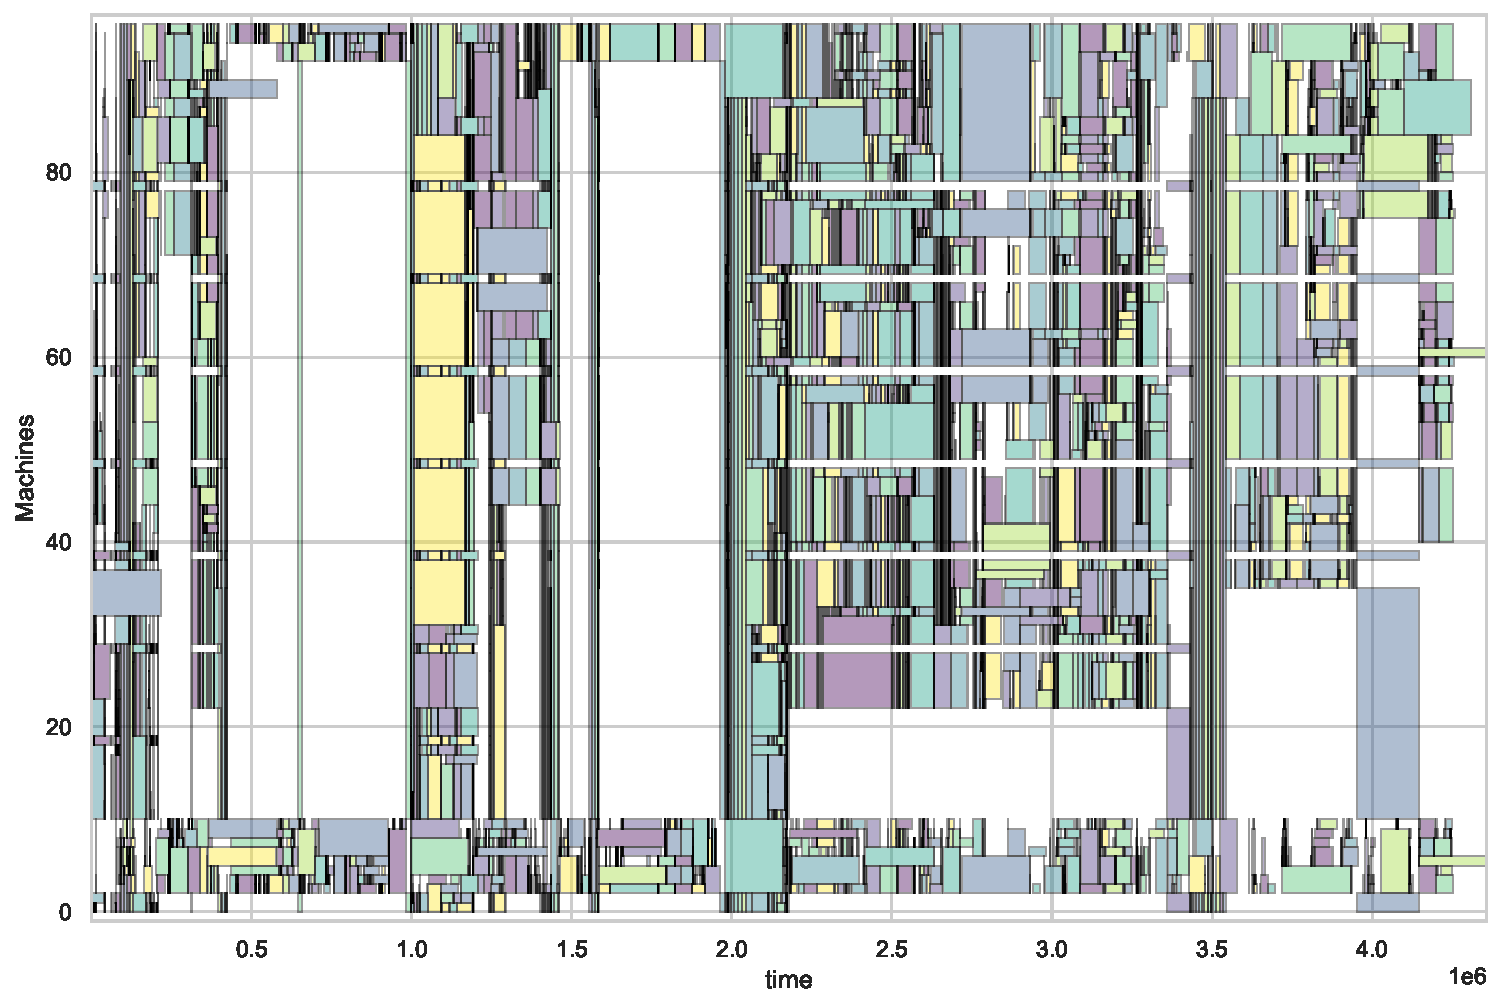
\includegraphics[width=\textwidth]{reservation_alloc-only_gantt_future_head.pdf}
    \caption{Gantt chart of the first 3500 jobs executed by the no-future-1 scheduling policy in the Alloc-Only model (there are 96 compute nodes in the simulated platform).}
    \label{fig:reservation_alloc-only_gantt_future_head}
\end{figure}

If we examine \autoref{fig:reservation_io-aware_waiting-time}, which is presenting waiting time statistics for the IO-Aware model, we do not find clear evidence for starvation. The mean waiting time of no-future-1 is smaller than fcfs. Plots of quantiles show similar dependencies for both models. There is no noticeable gap in the tail distribution. We also run these experiments for the split workloads. Their results are presented in \autoref{fig:reservation_alloc-only_parts_waiting-time} and  \autoref{fig:reservation_io-aware_parts_waiting-time}, respectively, for Alloc-Only and IO-Aware model. In \autoref{fig:reservation_alloc-only_parts_waiting-time}, no-future-1 for all the workload parts presents lower mean waiting time than fcfs, but with a varying difference. However, for \autoref{fig:reservation_io-aware_parts_waiting-time}, we see one case of a higher mean waiting time (Workload 13). We conclude that the significant starvation effect rarely occurs for no-future-1 schedule, but when it does, it may considerably deteriorate scheduling performance.

In terms of backfill-1 and filler, we can observe that for both models, the first one has a smaller mean waiting time, higher median and similar distribution presented by other quantiles. Tail distribution plots show substantially more outliers for filler, which is expected as it is not a fair scheduling algorithm by definition.

\paragraph{Turnaround time, slowdown and bounded slowdown}
For turnaround time, we may see similar relations between scheduling algorithms as for waiting time. Naturally, the median has higher values, so all quantiles are distinguishable in the quantiles plots.

In terms of slowdown and bounded slowdown, both backfill-1 and filler have relatively low means and medians close to $1$. The most dominate difference can be noticed for fcfs in the tail distribution. For slowdown, there are multiple outlying values, which do not occur for bounded slowdown. It suggests that fcfs could significantly delay short jobs. Nevertheless, no-future-1 have extensively more outliers for both slowdown and bounded slowdown than fcfs. Those conclusions apply for both models.

\paragraph{Waiting queue load}
Compute load and storage load plots, shown in \autoref{fig:reservation_alloc-only_compute-load}, \autoref{fig:reservation_alloc-only_storage-load} \autoref{fig:reservation_io-aware_compute-load} and \autoref{fig:reservation_io-aware_storage-load}, present the summarised number of processors and burst buffer size requested by all jobs that are in the waiting queue at a given moment. The meaning of lines on the plots is following:
\begin{itemize}
    \item Orange - total amount of resources available in the platform
    \item Blue - summarised resource requirements from jobs in the queue
    \item Dotted green - mean resource requirement (may differ from other plots due to number rounding)
    \item Red vertical lines at the bottom - queue reset events (situation when the the waiting queue was empty)
\end{itemize}

We may observe, by an increase in the compute load, that for backfill-1 and filler schedules, the last job submission happened just before the simulation end. Therefore, we conclude that our workloads were correctly calibrated for online scheduling.

Compute and storage load plots are visually similar for corresponding schedules. It may suggest that compute load and storage load are highly correlated in the workloads.

\paragraph{Conclusion}
Our results indicate that \textbf{backfilling without future reservations of burst buffers (no-future-1) may significantly deteriorate the efficiency of job scheduling} in terms of waiting time and slowdown. In extreme cases, \textbf{backfilling without future reservations of burst buffers may result in even higher mean waiting time than first-come-first-served scheduling without any backfilling}. Furthermore, \textbf{backfilling without future reservations of burst buffers is not a fair sharing policy} as it effects with an enormous number of arbitrarily delayed jobs. Its tail distribution of bounded slowdown shows a very high number of outliers.

% \FloatBarrier
% \clearpage

\subsection{Alloc-Only model}
\begin{figure}[hp]
    \centering
    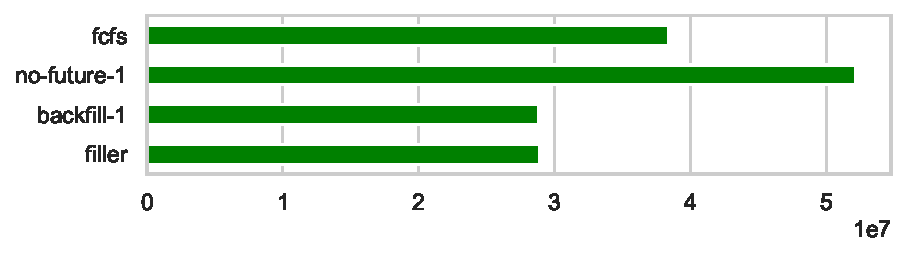
\includegraphics[width=\textwidth]{reservation_alloc-only_makespan.pdf}
    \caption{Makespan}
    \label{fig:reservation_alloc-only_makespan}
\end{figure}

\begin{figure}[hp]
    \centering
    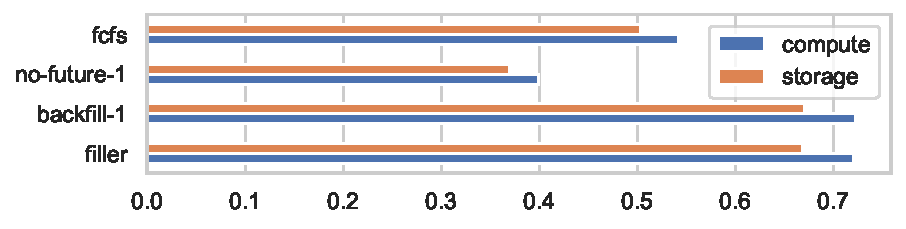
\includegraphics[width=\textwidth]{reservation_alloc-only_utilisation.pdf}
    \caption{System utilisation}
    \label{fig:reservation_alloc-only_utilisation}
\end{figure}

\resplot{alloc-only}{waiting-time}{Waiting time}
\resplot{alloc-only}{turnaround-time}{Turnaround time}
\resplot{alloc-only}{slowdown}{Slowdown}
\resplot{alloc-only}{bounded-slowdown}{Bounded slowdown}

% \begin{figure}[p]
%     \centering
%     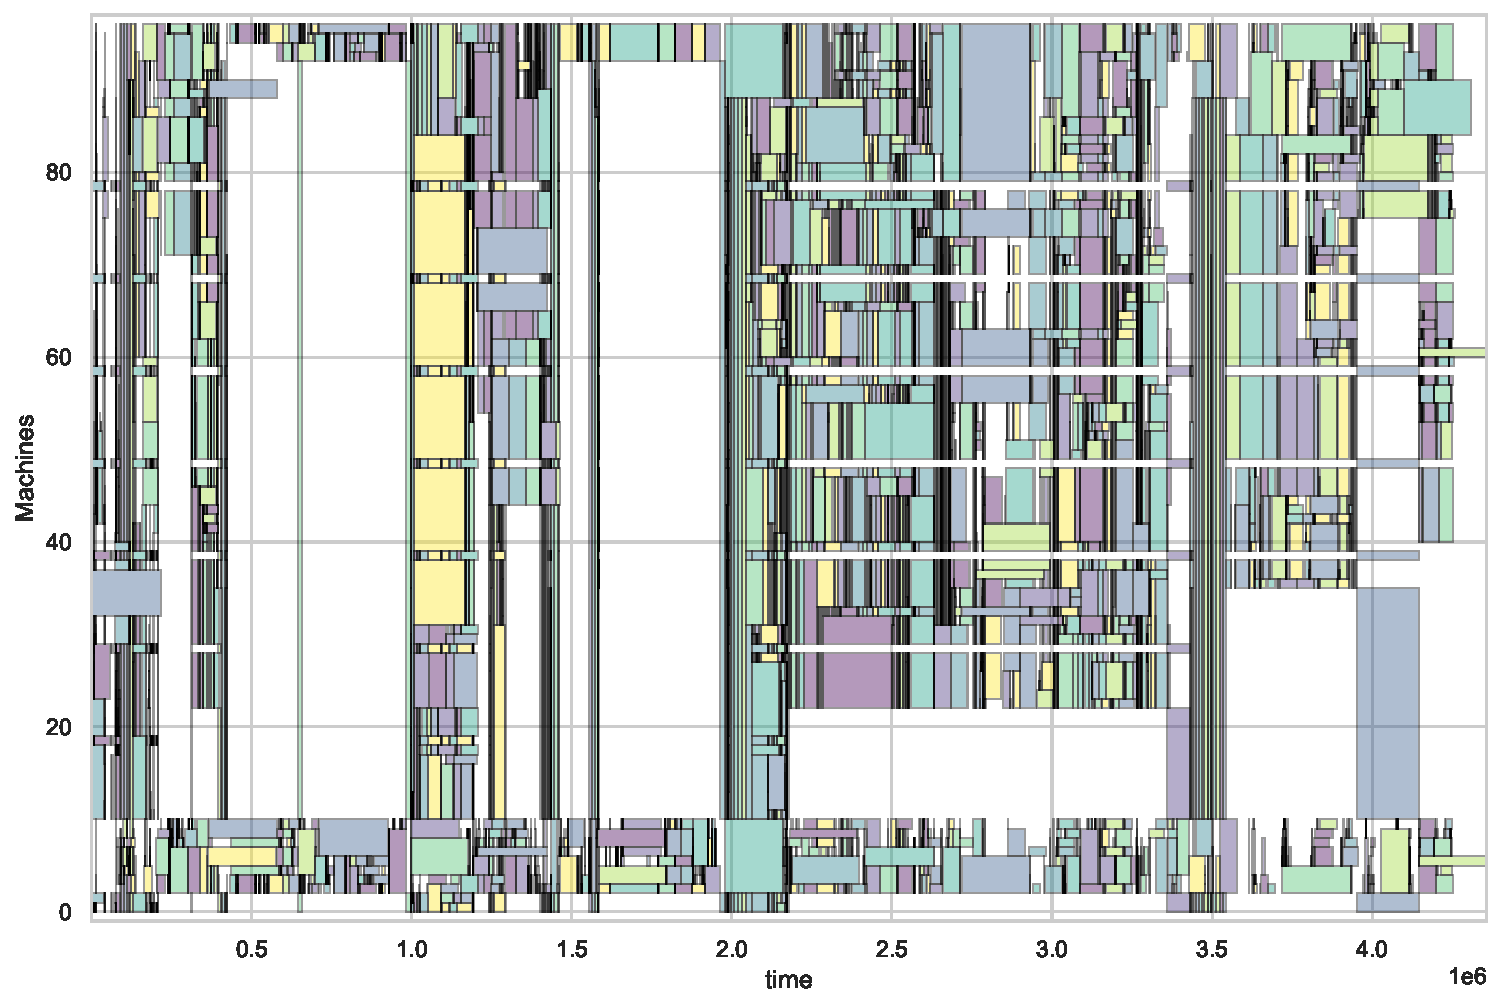
\includegraphics[width=\textwidth]{reservation_alloc-only_gantt_future_head.pdf}
%     \caption{Gantt chart of the first 3500 jobs executed by the no-future-1 scheduling policy}
%     \label{fig:reservation_alloc-only_gantt_future_head}
% \end{figure}

% \begin{figure}[p]
%     \centering
%     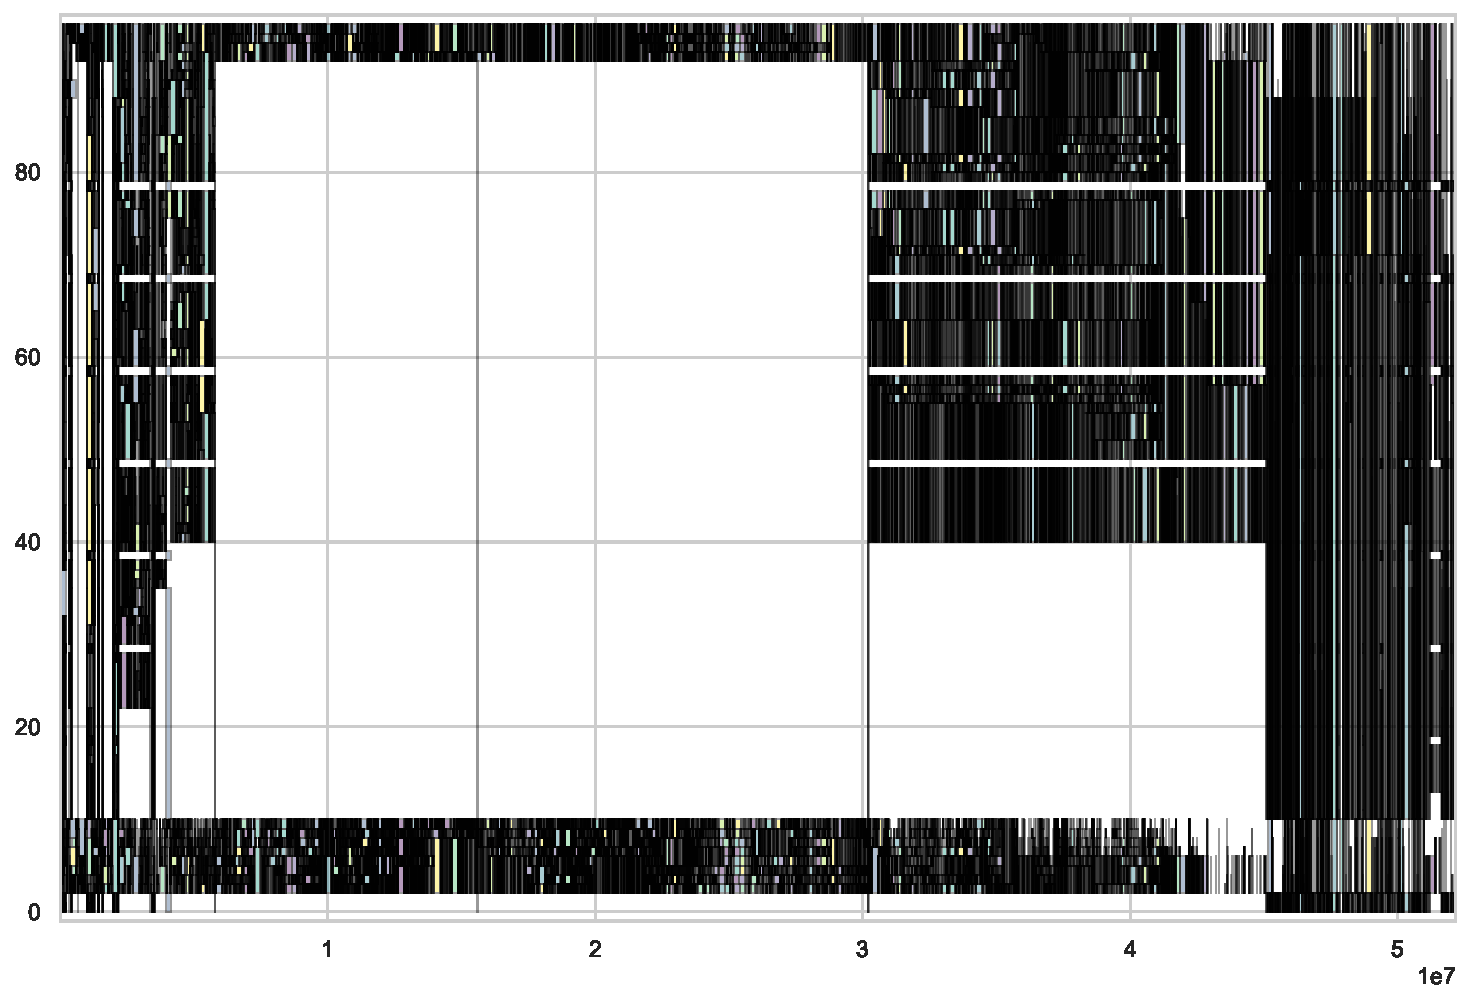
\includegraphics[width=\textwidth]{reservation_alloc-only_gantt_future.pdf}
%     \caption{Gantt chart}
%     \label{fig:reservation_alloc-only_gantt_future}
% \end{figure}

% \begin{figure}[p]
%     \centering
%     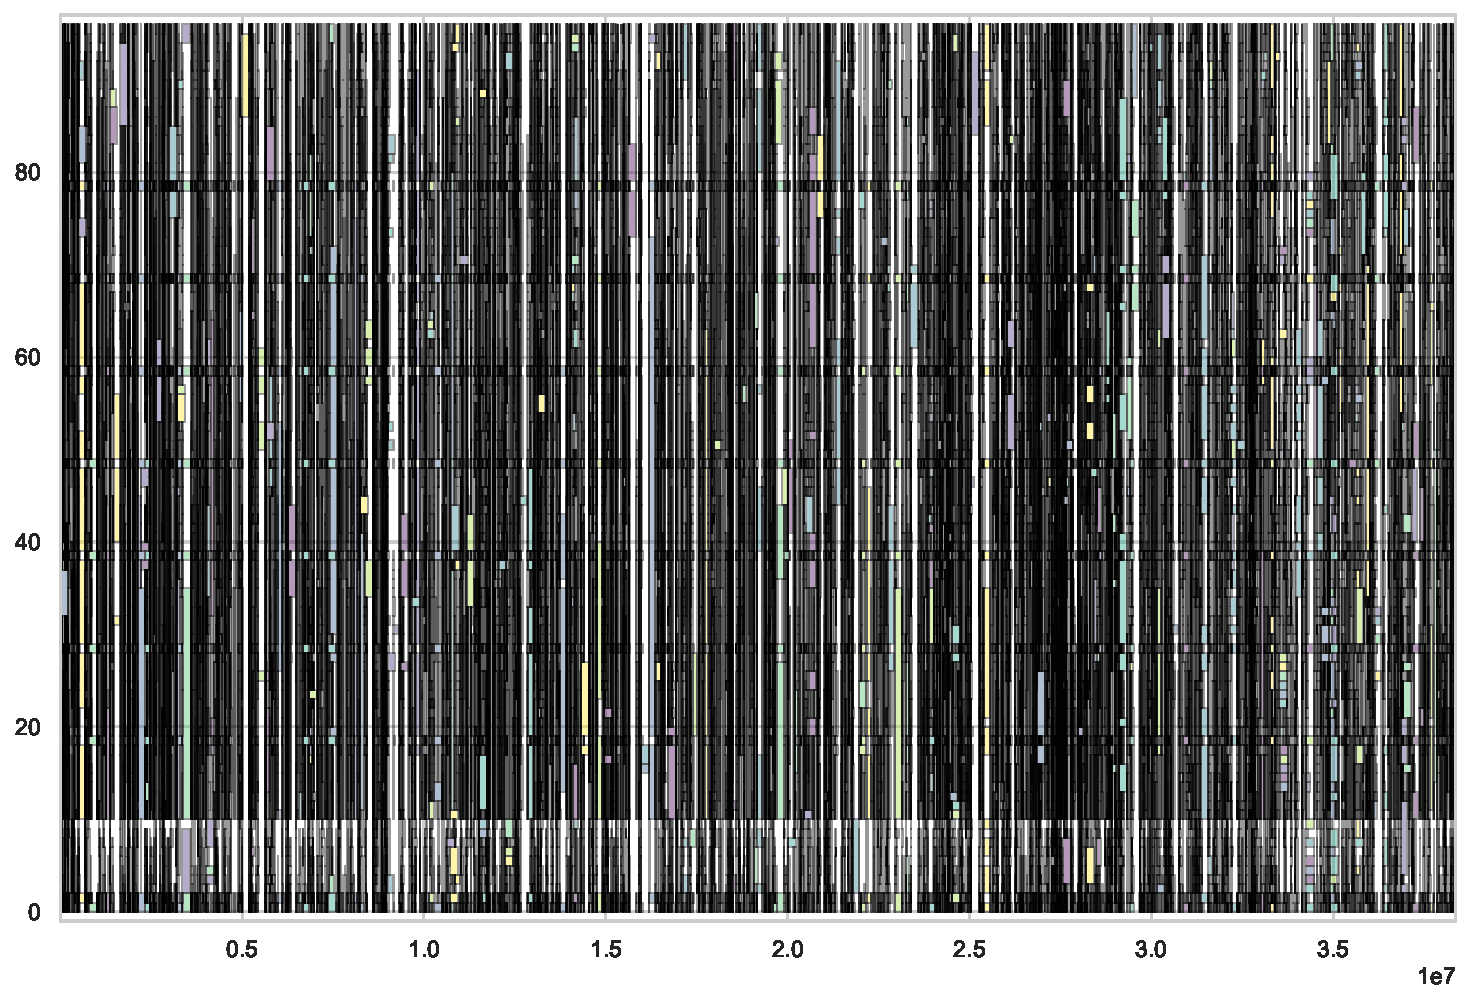
\includegraphics[width=\textwidth]{reservation_alloc-only_gantt_fcfs.pdf}
%     \caption{Gantt chart}
%     \label{fig:reservation_alloc-only_gantt_fcfs}
% \end{figure}

% \begin{figure}[p]
%     \centering
%     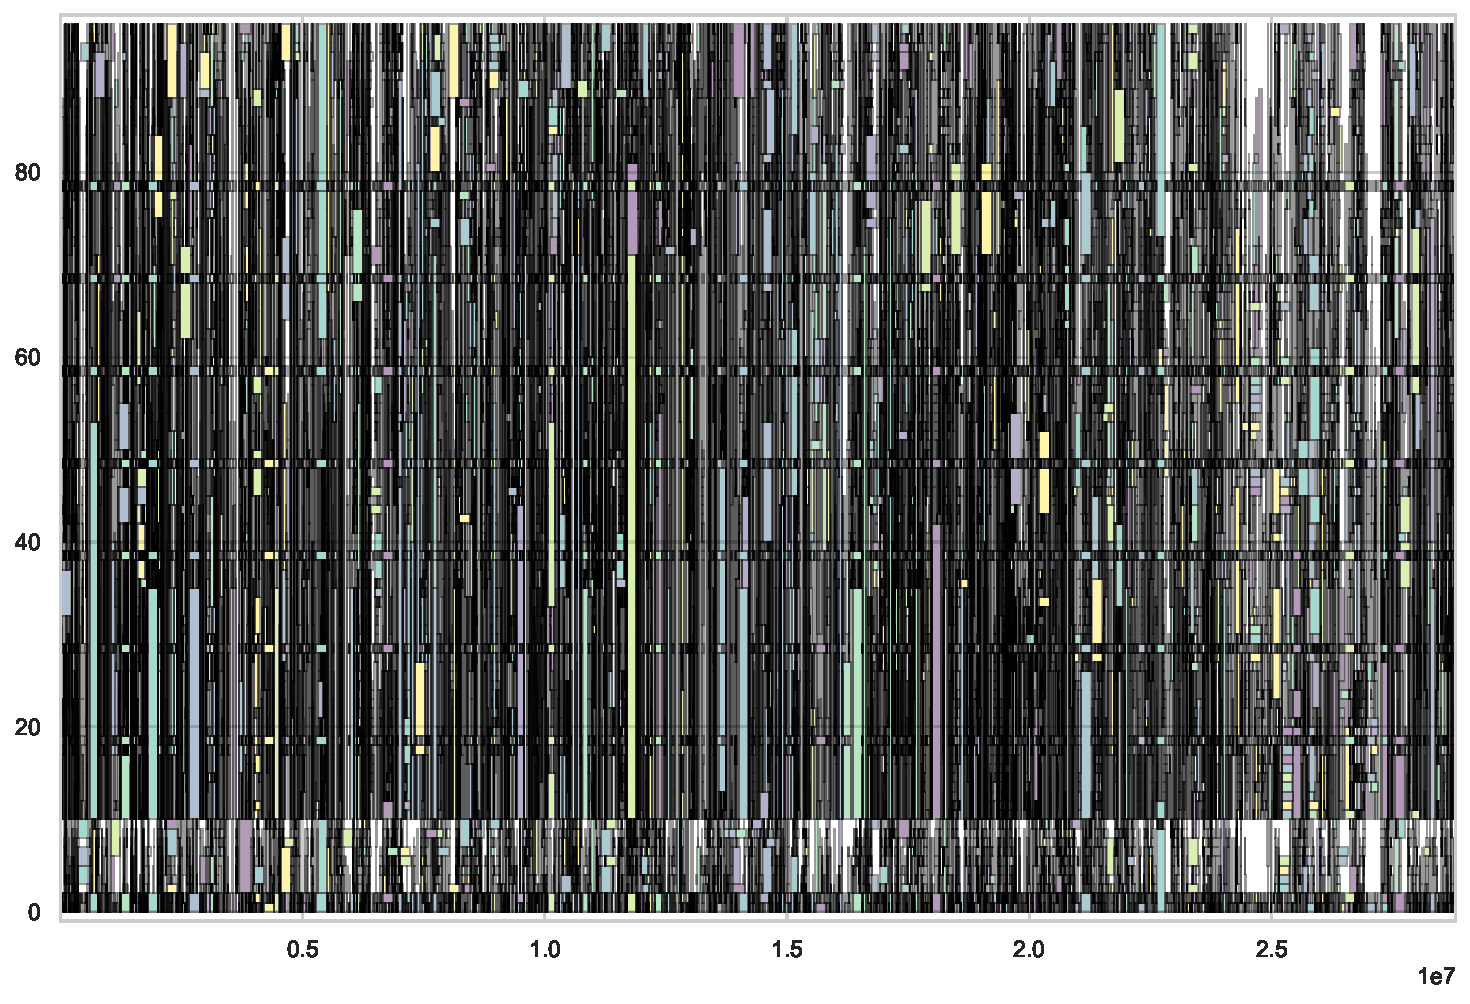
\includegraphics[width=\textwidth]{reservation_alloc-only_gantt_backfill-1.pdf}
%     \caption{Gantt chart}
%     \label{fig:reservation_alloc-only_gantt_backfill-1}
% \end{figure}

\loadplot{alloc-only}{compute-load}{Compute load (different axes ranges)}
\loadplot{alloc-only}{storage-load}{Storage load (different axes ranges)}

\begin{figure}[p]
    \centering
    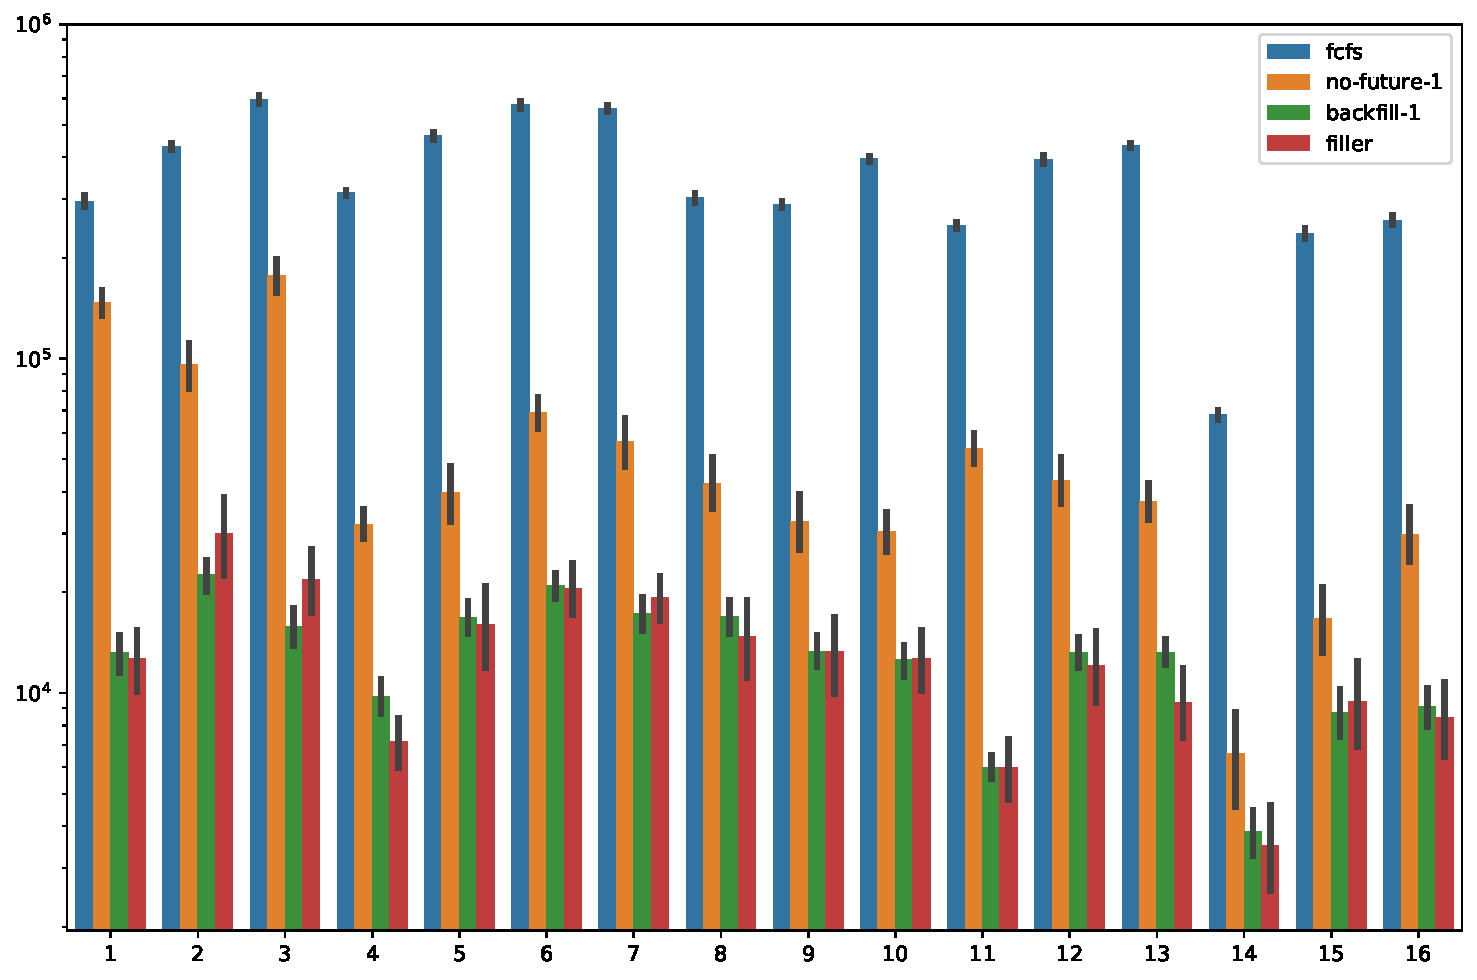
\includegraphics[width=\textwidth]{reservation_alloc-only_parts_waiting-time.pdf}
    \caption{Mean waiting time of the split workload}
    \label{fig:reservation_alloc-only_parts_waiting-time}
\end{figure}

\begin{figure}[p]
    \centering
    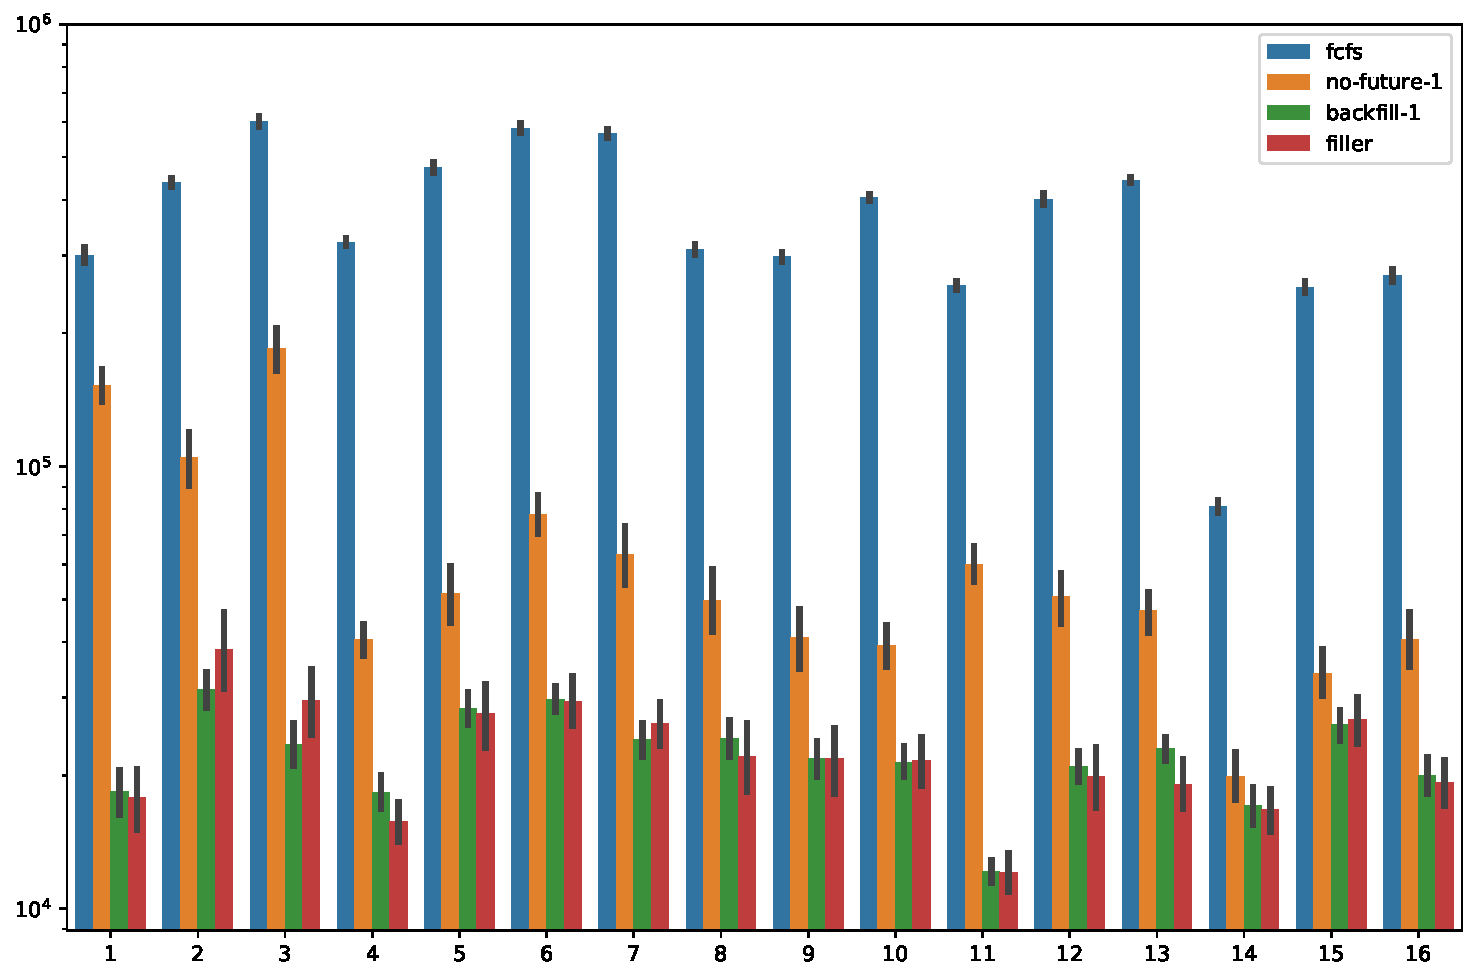
\includegraphics[width=\textwidth]{reservation_alloc-only_parts_turnaround-time.pdf}
    \caption{Mean turnaround time of the split workload}
    \label{fig:reservation_alloc-only_parts_turnaround-time}
\end{figure}

\begin{figure}[p]
    \centering
    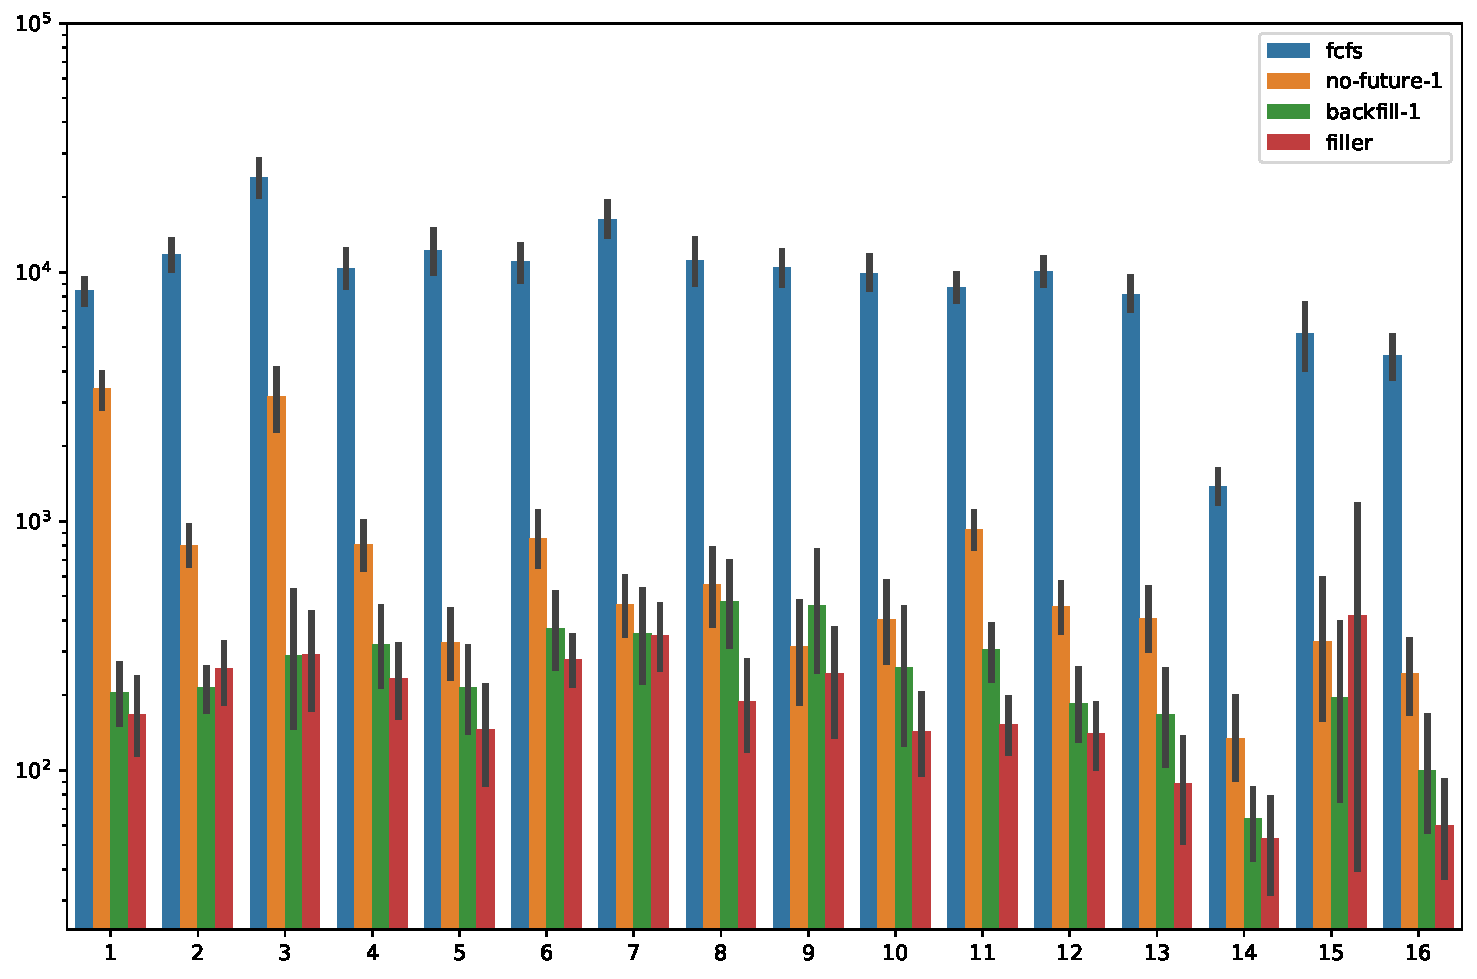
\includegraphics[width=\textwidth]{reservation_alloc-only_parts_slowdown.pdf}
    \caption{Mean slowdown of the split workload}
    \label{fig:reservation_alloc-only_parts_slowdown}
\end{figure}

\begin{figure}[p]
    \centering
    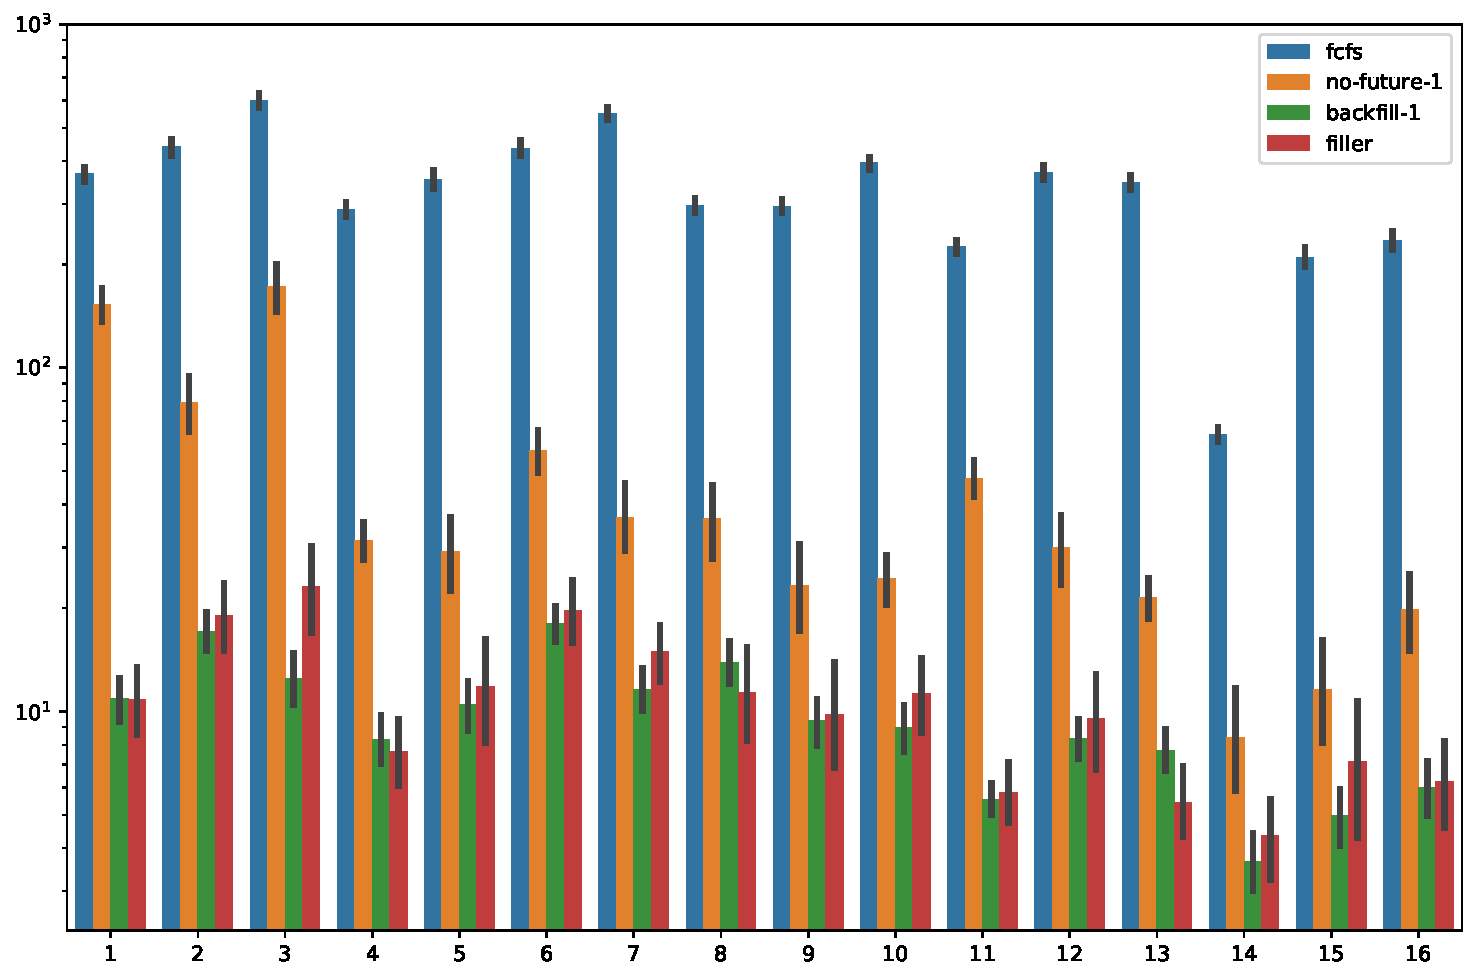
\includegraphics[width=\textwidth]{reservation_alloc-only_parts_bounded-slowdown.pdf}
    \caption{Mean bounded slowdown of the split workload}
    \label{fig:reservation_alloc-only_parts_bounded-slowdown}
\end{figure}

\FloatBarrier

\subsection{IO-Aware model}
\begin{figure}[hp]
    \centering
    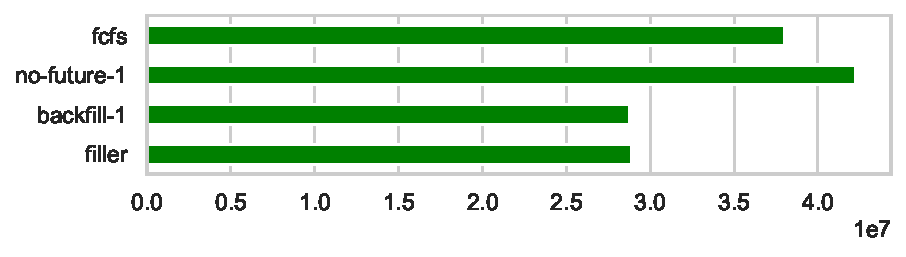
\includegraphics[width=\textwidth]{reservation_io-aware_makespan.pdf}
    \caption{Makespan}
    \label{fig:reservation_io-aware_makespan}
\end{figure}

\begin{figure}[hp]
    \centering
    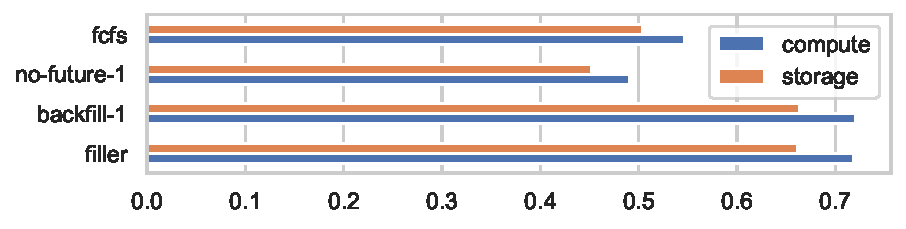
\includegraphics[width=\textwidth]{reservation_io-aware_utilisation.pdf}
    \caption{System utilisation}
    \label{fig:reservation_io-aware_utilisation}
\end{figure}

\resplot{io-aware}{waiting-time}{Waiting time}
\resplot{io-aware}{turnaround-time}{Turnaround time}
\resplot{io-aware}{slowdown}{Slowdown}
\resplot{io-aware}{bounded-slowdown}{Bounded slowdown}

\loadplot{io-aware}{compute-load}{Compute load (different axes ranges)}
\loadplot{io-aware}{storage-load}{Storage load (different axes ranges)}

\begin{figure}[p]
    \centering
    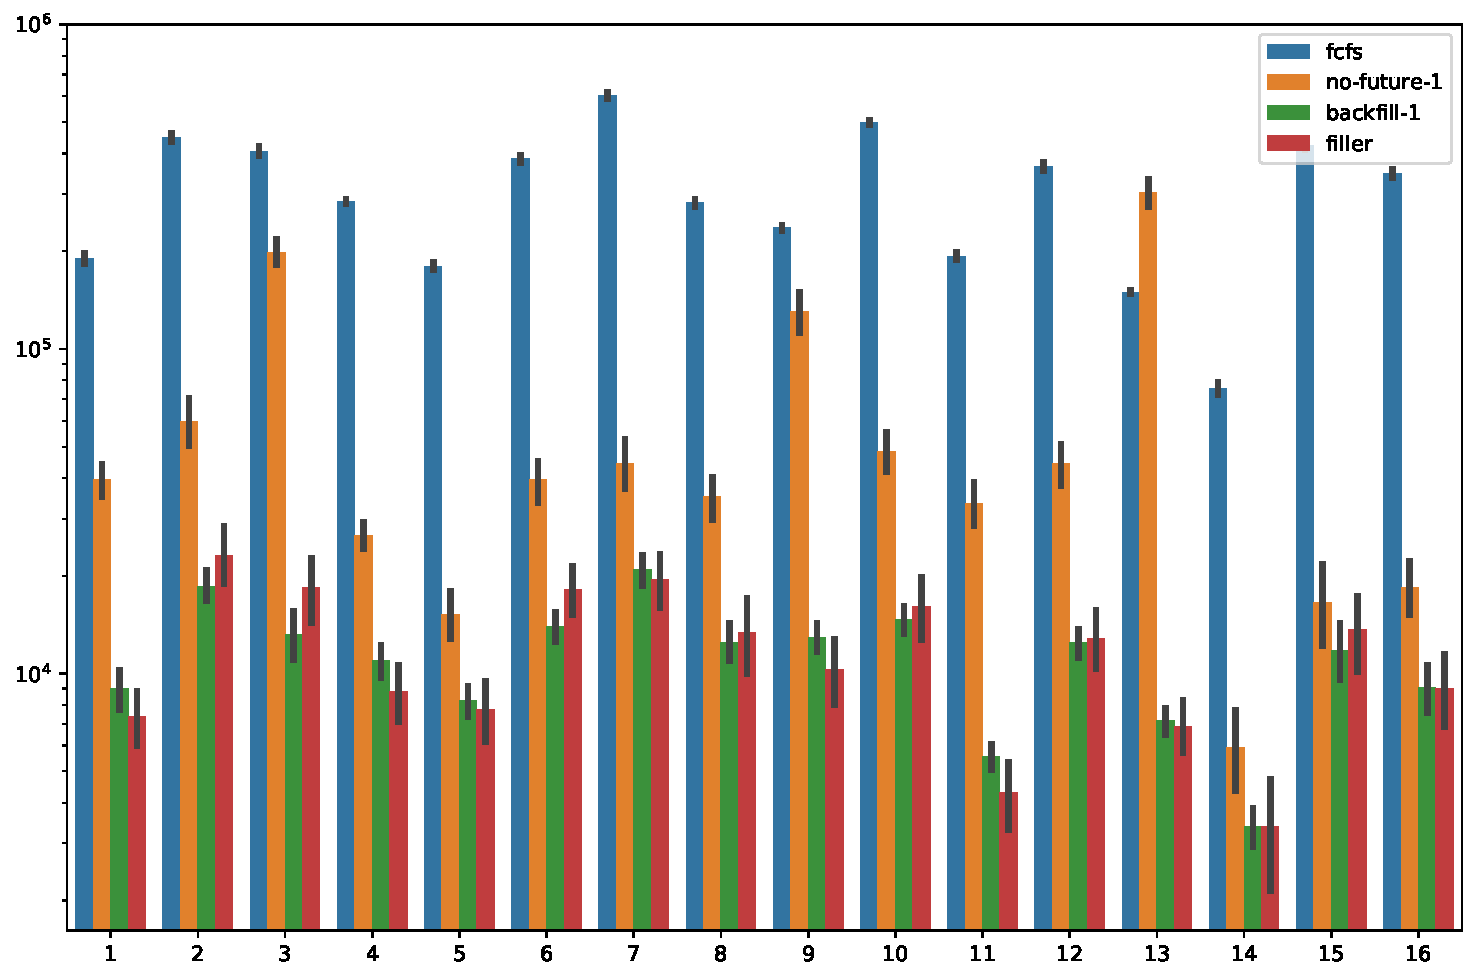
\includegraphics[width=\textwidth]{reservation_io-aware_parts_waiting-time.pdf}
    \caption{Mean waiting time of the split workload}
    \label{fig:reservation_io-aware_parts_waiting-time}
\end{figure}

\begin{figure}[p]
    \centering
    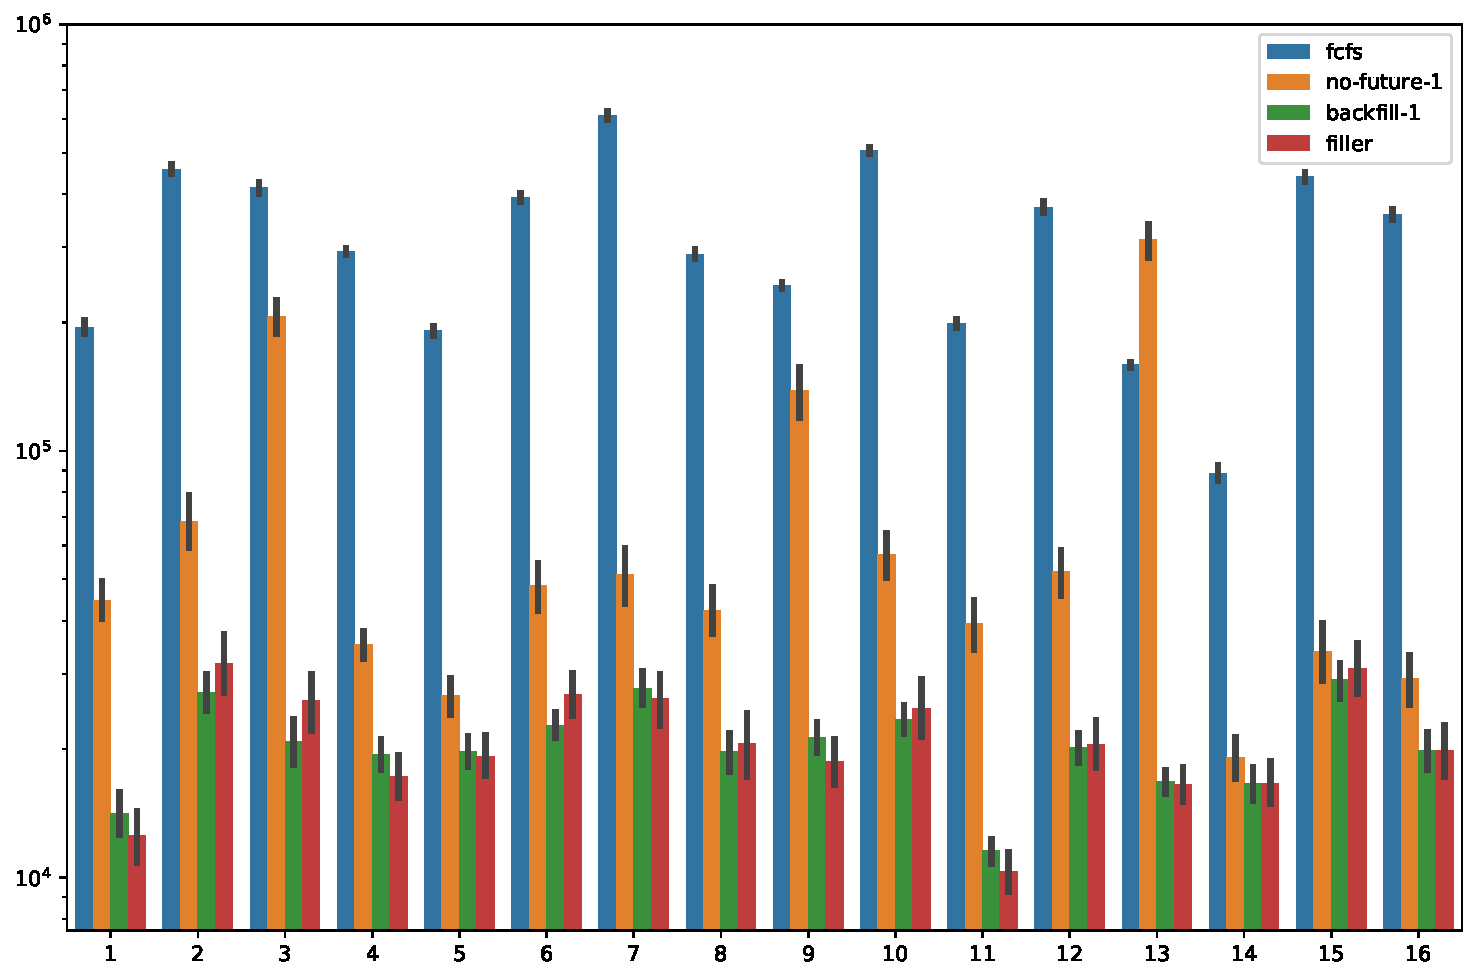
\includegraphics[width=\textwidth]{reservation_io-aware_parts_turnaround-time.pdf}
    \caption{Mean turnaround time of the split workload}
    \label{fig:reservation_io-aware_parts_turnaround-time}
\end{figure}

\begin{figure}[p]
    \centering
    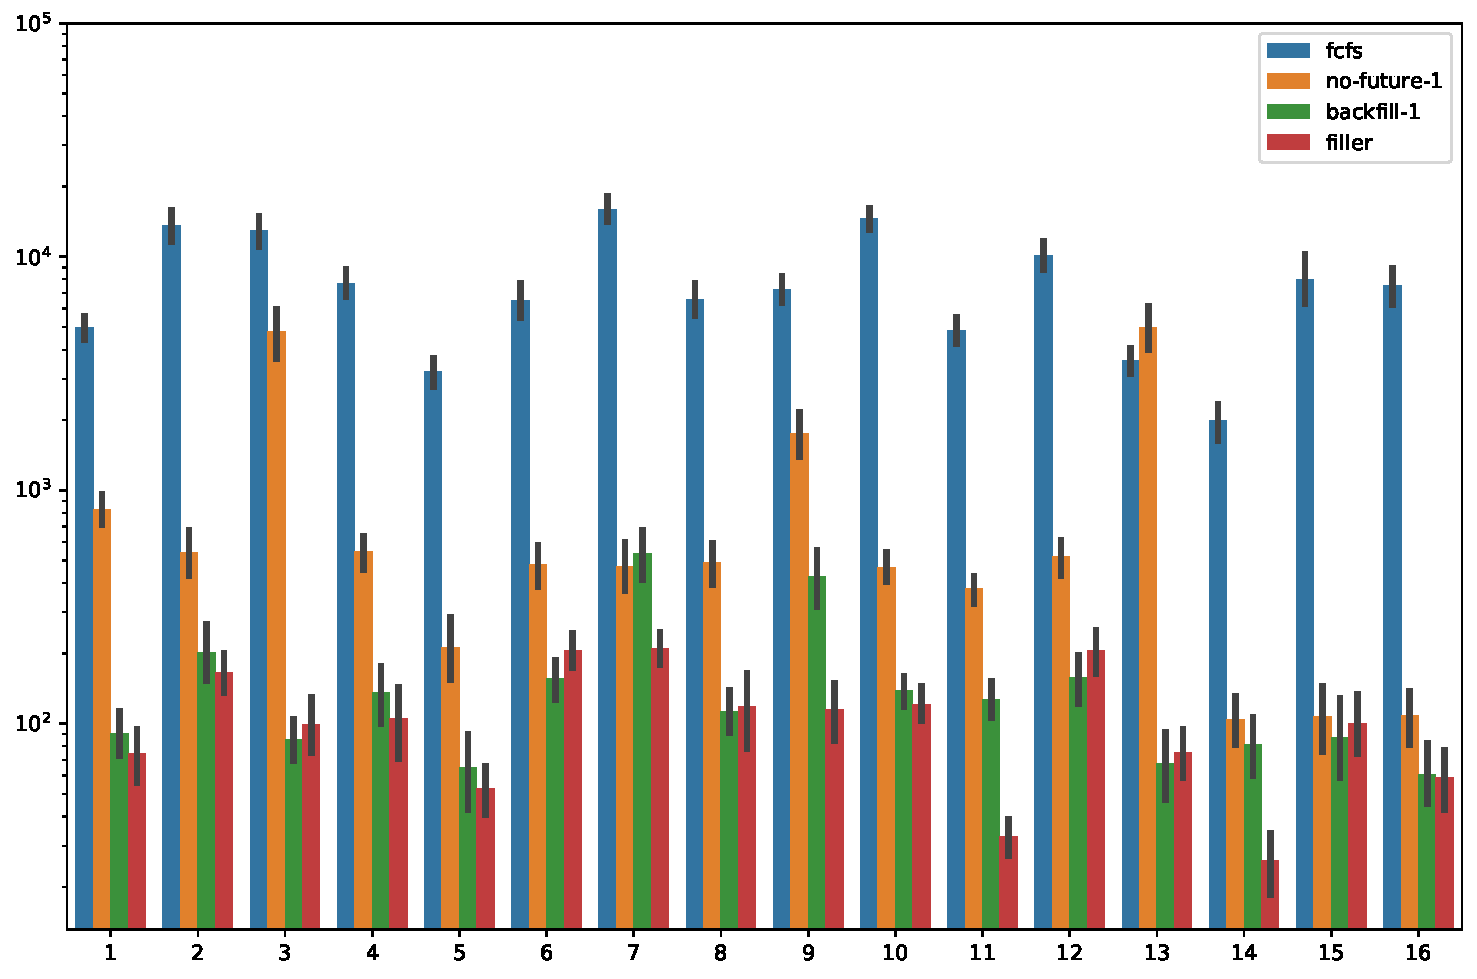
\includegraphics[width=\textwidth]{reservation_io-aware_parts_slowdown.pdf}
    \caption{Mean slowdown of the split workload}
    \label{fig:reservation_io-aware_parts_slowdown}
\end{figure}

\begin{figure}[p]
    \centering
    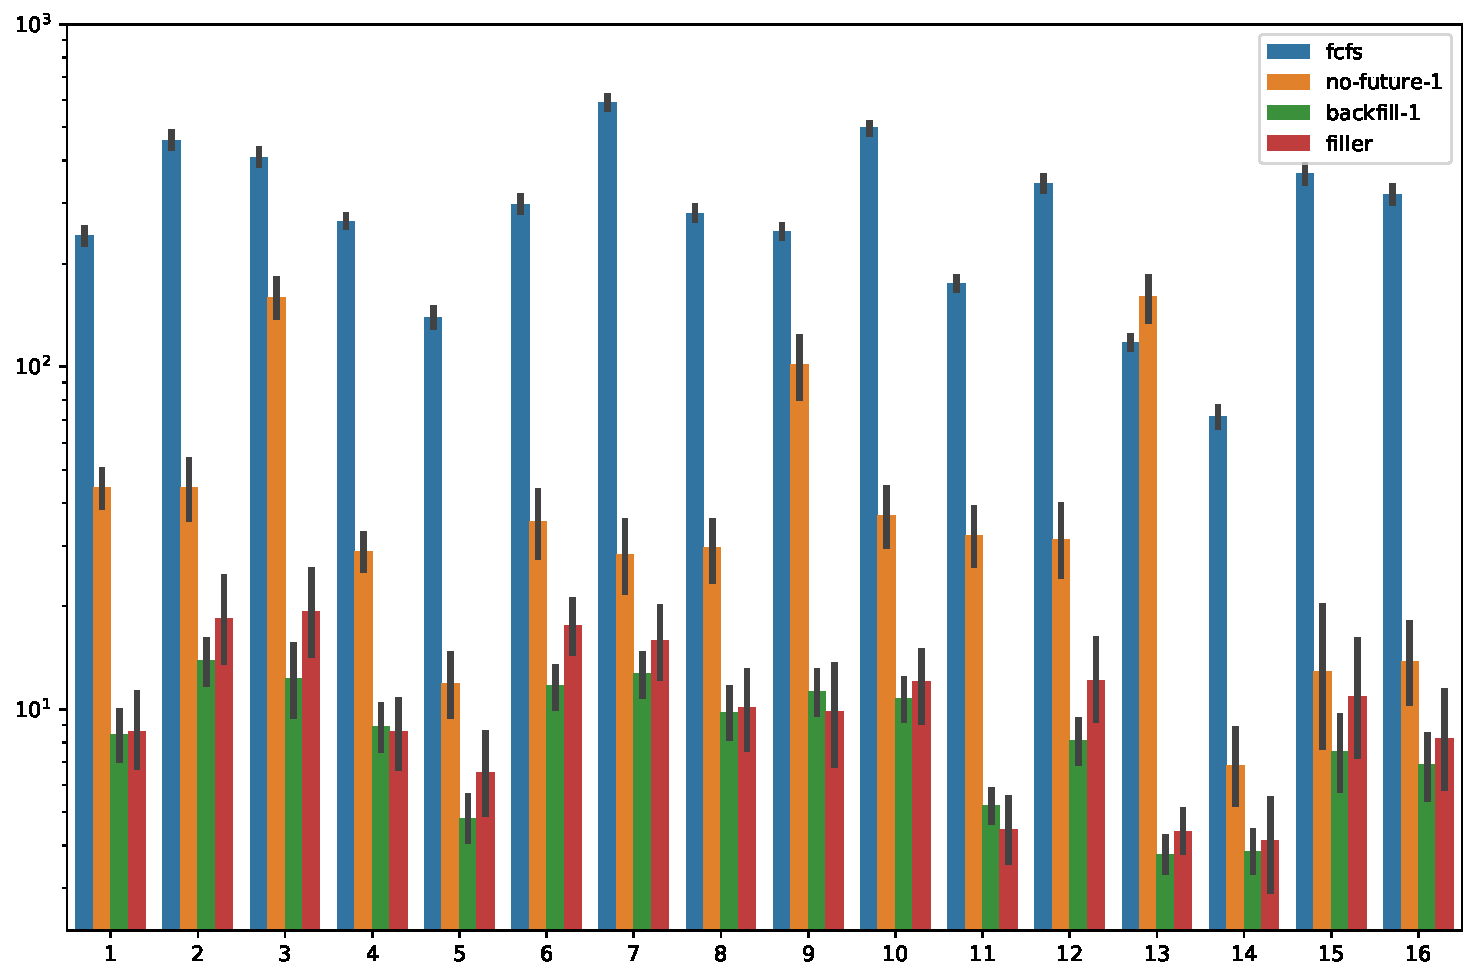
\includegraphics[width=\textwidth]{reservation_io-aware_parts_bounded-slowdown.pdf}
    \caption{Mean bounded slowdown of the split workload}
    \label{fig:reservation_io-aware_parts_bounded-slowdown}
\end{figure}

\FloatBarrier

\section{System utilisation maximising scheduling} \label{sec:maxutil-results}
We dedicate this section for finding the optimal \emph{balance factor} $\beta$ for Maxutil algorithm shown in listing \ref{alg:maxutil}. As described in \autoref{sec:maxutil}, the value of $\beta$ determines how likely is the algorithm to reduce either compute or storage load. We test four different values of $\beta$: $0.5$ (maxutil-0.5-1, green), $1$ (maxutil-1-1, red), $1.5$ (maxutil-1.5-1, purple), $2$ (maxutil-2-1, brown). We compare these schedules with two canonical scheduling algorithms: First-Come-First-Served backfilling (backfill-1, blue) and Shortest-Job-First backfilling (backfill-sjf-1, orange). For all experiments we set the \emph{reservation depth} $D$ to $1$, which ensures the fairness property. The \emph{maximum number of steps for hill climbing} $N$ is $5000$ in each case, as stated in \autoref{sec:maxutil}.

From \autoref{fig:maxutil_waiting-time}, we see that all scheduling policies except backfill-1 have similar mean waiting time. Mean waiting time of backfill-1 is slightly higher than the others. The quantile plot also presents similar scores for all schedules, except for backfill-sjf-1, for which the last 32-quantile is higher than other. In terms of tail distribution, maxutil-1.5-1 and maxutil-2-1 have more significantly outlying waiting times than others. However, all the above differences are relatively small, so we find that waiting time does not indicate the optimal value for $\beta$.

Plots for turnaround time in \autoref{fig:maxutil_turnaround-time} presents the same relations as the waiting time.

For slowdown, backfill-sjf-1 shows significant improvement in all compared statistics.This improvement, however, does not transit to bounded slowdown. It shows only a slight decrease in mean in favour of the backfill-sjf-1. The schedule backfill-1 achieves higher mean and quantile statistics than the other schedules. For all values of $\beta$, maxutil schedules present negligible differences in bounded slowdown based statistics.

For the IO-Aware model with the full workload, we did not found any vital differences in scheduling results for the Maxutil algorithms depending on the \emph{balance factor} $\beta$. Therefore, for comparing Maxutil with other algorithms in the following sections, we use the default value of $\beta=1$.

% \clearpage

\maxutilplot{waiting-time}{Waiting time}
\maxutilplot{turnaround-time}{Turnaround time}
\maxutilplot{slowdown}{Slowdown}
\maxutilplot{bounded-slowdown}{Bounded slowdown}

\FloatBarrier

\section{Window-based combinatorial scheduling} \label{sec:window-results}
The main parameter in Algorithm \ref{alg:window} is the \emph{max window size} $N$. A different approach to window-based scheduling was explored in \cite{10.1145/3307681.3325401}. Experiments there were performed for window size ranging from $1$ to $20$. We were, unfortunately, unable to test our approach for the window size greater than $10$ due to a multi-threading issue in one of our software dependencies - Z3 Solver. Therefore, we only test the influence of resource reservation on the algorithm for a fixed $N=10$. We compare the following scheduling policies:
\begin{itemize}
    \item FCFS backfilling (backfill-1, blue)
    \item SJF backfilling (backfill-sjf-1)
    \item Window-based combinatorial scheduling with a reservation of the first job in the queue (window-1, green)
    \item Window-based combinatorial scheduling without resource reservations (window-0, red)
\end{itemize}

In terms of waiting time and turnaround time, window-1 presents almost identical statistics as backfill-sjf-1. Whereas, window-0 show better results in quantiles, but much higher mean. This schedule is less restrictive than window-1 as it does not implement any fairness mechanism. The value of the mean could be easily explained by the tail distribution, where we see many outliers for window-0, which may evince starvation of jobs.

For bounded slowdown, there can be distinguished ordering between the algorithms. 
The best results are achieved by backfill-sjf-1. Then window-1 shows better results than backfill-1. While window-0 has significantly worse mean than all other algorithms.

For the following sections, we select window-1 for comparison as window-0 does not provide fair sharing.

\windowplot{waiting-time}{Waiting time}

\windowplot{turnaround-time}{Turnaround time}
\windowplot{slowdown}{Slowdown}
\windowplot{bounded-slowdown}{Bounded slowdown}

\FloatBarrier

\section{Plan-based scheduling} \label{sec:plan-results}
In this section, we study multiple variants of plan-based scheduling introduced in \autoref{sec:plan}. Our goal is to test how resource reservations and optimisation objectives influence the overall efficiency of scheduling. As mentioned in \autoref{sec:methodology}, we present results of simulations for only IO-Aware model. We compare the set of the following policies:
\begin{itemize}
    \item FCFS EASY-backfilling (backfill-1, blue)
    \item SJF EASY-backfilling (backfill-sjf-1, orange)
    \item Plan-based (plan-sum-1, green)
    \begin{itemize}
        \item reservation of resources for the first job ($D=1$)
        \item minimise the sum of waiting time ($\alpha=1$)
    \end{itemize}
    \item Plan-based (plan-square-1, red)
    \begin{itemize}
        \item reservation of resources for the first job ($D=1$)
        \item minimise the sum of squared waiting time ($\alpha=2$)
    \end{itemize}
    \item Plan-based (plan-start-1, purple)
    \begin{itemize}
        \item reservation of resources for the first job ($D=1$)
        \item minimise starting time of the latest job
    \end{itemize}
    \item Plan-based (plan-sum-0, brown)
    \begin{itemize}
        \item no reservations ($D=0$)
        \item minimise the sum of waiting time ($\alpha=1$)
    \end{itemize}
    \item Plan-based (plan-square-0, pink)
    \begin{itemize}
        \item no reservations ($D=0$)
        \item minimise the sum of squared waiting time ($\alpha=2$)
    \end{itemize}
    \item Plan-based (plan-cube-0, grey)
    \begin{itemize}
        \item no reservations ($D=0$)
        \item minimise the sum of cubed waiting time ($\alpha=3$)
    \end{itemize}
    \item Plan-based (plan-start-0, gold)
    \begin{itemize}
        \item no reservations ($D=0$)
        \item minimise starting time of the latest job
    \end{itemize}
\end{itemize}

\paragraph{Waiting time and turnaround time}
All scheduling algorithms with resource reservations achieve comparable results in mean waiting time. They, however, differ in ordered statistics. Plan-sum-1, plan-square-1 and plan-start-1 are visibly better in the last and last but one quantile than backfill-sjf-1. Further relations between them are hard to distinguish as plan-square-1 has better distribution for the last quantile but worse for others compared to plan-sum-1 and plan-start-1. The tail distribution shows no outstanding results for all of these schedules. The especially interesting observation is that plan-sum-1 and plan-start-1 demonstrate an almost identical outcome. For turnaround time, all these relations remain accurate.

The next subset of scheduling policies with similar results is plan-sum-0 and plan-start-0. As we indicated in \autoref{sec:plan}, they do not implement any fair sharing mechanism. We can see the confirmation of this fact in \autoref{fig:plan_waiting-time_dist}, where that both expose a significant number of outliers in waiting time statistic. These outliers explain very high mean waiting time achieved by both schedules. For distribution of quantiles, plan-sum-0 and plan-start-0 show better results than policies with reservation but are only comparable with plan-square-0 and plan-cube-0. To summarise, plan-sum-0 and plan-start-0 are not practical candidates for implementation in a real RJMS.

Lastly, plan-square-0 and plan-cube-0 are present considerably lower mean waiting and turnaround time than other algorithms. Compared to scheduling policies with resource reservations, plan-square-0 and plan-cube-0 have a few outstanding values. However it is relatively negligible when compared to the distribution of plan-sum-0 and plan-start-0. Plan-square-0 achieves slightly better results in mean and quantiles than plan-cube-0.

\paragraph{Slowdown and bounded slowdown}
For mean slowdown, the best results are presented by backfill-sjf-1, plan-sum-0, plan-square-0, plan-cube-0 and plan-start-0. However, it does not hold for the bounded slowdown, for which plan-square-0 is better than all other algorithms. Plan-cube-0 follows its score. The value of mean is not reflected by the quantiles plots (\autoref{fig:plan_slowdown_boxen}, \autoref{fig:plan_bounded-slowdown_boxen}), where the best distributions are presented by plan-sum-0 and plan-start-0 for both slowdown and bounded slowdown. The tail distribution of slowdown shows similar results for all algorithms. For bounded slowdown, tail distribution presents a few highly outstanding values only for plan-sum-0 and plan-start-0, yet there are considerably fewer outliers that for waiting time.

\paragraph{Conclusion}
Plan-based scheduling algorithms with resource reservations do not demonstrate better results than the canonical scheduling algorithms with burst buffer reservations. Plan-sum-0 and plan-start-0 proved that they lack a fairness mechanism and consequently can arbitrarily delay jobs in the waiting queue. Similarly, plan-square-0 and plan-cube-0 do not implement any strict mechanism for ensuring fairness. However, in the experiments, they did not indicate any relevantly outlying values in waiting time. Therefore, we consider plan-square-0 and plan-cube-0 as the best scheduling algorithms discussed in this section as they showed significant improvement in the mean and remarkable distribution for all statistics. Furthermore, plan-square-0 was slightly better than plan-cube-0 in all measurements.

\planplot{waiting-time}{Waiting time}
\planplot{turnaround-time}{Turnaround time}
\planplot{slowdown}{Slowdown}
\planplot{bounded-slowdown}{Bounded slowdown}

\FloatBarrier

\section{Comparison of the best scheduling algorithms} \label{sec:best}
From previous sections, we select scheduling policies that showed the best results for each algorithm. We compare them based on the in-depth analysis performed for both Alloc-Only and IO-Aware model. For each selected algorithm, we present the results for full workloads and split workloads. The selected algorithms are:
\begin{itemize}
    \item FCFS EASY-backfilling (backfill-1, blue)
    \item SJF EASY-backfilling (backfill-sjf-1, orange)
    \item Maxutil with \emph{balance factor} $\beta=1$ (maxutil-1.0-1, green)
    \item Window-based combinatorial scheduling with a reservation of the first job (window-1, red)
    \item Plan-based (plan-square-0, purple)
    \begin{itemize}
        \item no reservations ($D=0$)
        \item minimise the sum of squared waiting time ($\alpha=2$)
    \end{itemize}
    \item Plan-based (plan-cube-0, brown)
    \begin{itemize}
        \item no reservations ($D=0$)
        \item minimise the sum of cubed waiting time ($\alpha=3$)
    \end{itemize}
\end{itemize}
% In the first order we discuss results for 

\paragraph{Alloc-Only model}
In Sections \ref{sec:maxutil-results}, \ref{sec:window-results}, \ref{sec:plan-results}, we compared algorithms based on only the IO-Aware model. We supplement those results with experiments performed for the Alloc-Only model. Comparison of the results for both models provides us with information on the influence of I/O contentions and I/O congestion effects on burst buffer aware job scheduling.

The first outstanding observation is that backfill-sjf-1 for the full workload demonstrates worse results for mean and distribution of waiting time than backfill-1 (\autoref{fig:best_alloc-only_waiting-time}), which was not a case in the IO-Aware model. However, this relation is not reflected in \autoref{fig:best_alloc-only_parts_waiting-time}, presenting the mean waiting time for the split workload. For most of the parts, backfill-1 achieves worse results than backfill-sjf-1. Therefore, we find it probable that backfill-sjf-1 for the full workload was affected by unfavourable interlace of jobs.

Focusing on scheduling algorithms which optimise resource utilisation, we observe that maxutil-1.0-1 and window-1 achieve almost identical results in mean and distribution of waiting and turnaround time. For slowdown and bounded slowdown, window-1 tend to present a better outcome for the full workload. In terms of the split workload, we do not see a strict relation between those schedules. Moreover, the confidence intervals indicate a considerable uncertainty of the results. For \autoref{fig:best_alloc-only_parts_bounded-slowdown}, the uncertainty level is so great that it is at the same order of magnitude as the mean slowdown for each part. Consequently, we find the results of the mean slowdown as unreliable. In general, backfill-1, backfill-sjf-1, maxutil-1.0-1, window-1 show comparable results. For a given statistic, there are visible differences between them for the full workload. In plots \ref{fig:best_alloc-only_parts_waiting-time}-\ref{fig:best_alloc-only_parts_bounded-slowdown}, it is, however, visible that their results interleave for various workload parts.

In \autoref{sec:plan-results}, we stated that plan-square-0 is the best plan-based scheduling algorithm based on the analysis of the full workload in the IO-Aware model. Plan-cube-0 directly followed its results. We observe the same relations for the Alloc-Only model. From summary statistics plots in figures \ref{fig:best_alloc-only_waiting-time}-\ref{fig:best_alloc-only_bounded-slowdown}, it is clear that plan-square-0 and plan-cube-0 dominate other schedules. Furthermore, for the slowdown and bounded slowdown, all algorithms present similar tail distributions. The only statistic for which plan-square-0 and plan-cube-0 show a deterioration is the tail distribution of waiting and turnaround time. However, they present only a few jobs that have higher values than outliers of other schedules.

\paragraph{IO-Aware model}
For the canonical scheduling algorithms backfill-1 and backfill-sjf-1, the results for the IO-Aware model are discussed in \autoref{sec:maxutil-results}. The plan-based algorithms plan-square-0 and plan-cube-0 are compared in \autoref{sec:plan-results}. For waiting time and turnaround time, we generally observe similar relations between algorithms as they are in the Alloc-Only model. That is backfill-1,  backfill-sjf-1, maxutil-1.0-1 and window-1 have comparable performance. Similarly, plan-square-0 and plan-cube-0 present a much better performance in summary statistics but worse results in the tail distributions. The results for the bounded slowdown are similar for IO-Aware and Alloc-Only models. The schedules backfill-sjf-1, maxutil-1.0-1 and window-1 are comparable, backfill-1 is slightly worse, and plan-based scheduling policies strictly dominate others. For slowdown, as we already noticed backfill-sjf-1 indicates excellent results that are comparable with plan-square-0 and plan-cube-0. Window-1 present considerably worse results and is followed by maxutil-1.0-1.

\paragraph{Normalised mean plots}
The bar plots presenting values of mean enables to determine whether or not one scheduling algorithm dominate another for a given statistic. However, they do not directly inform if one algorithm is on average better than another. For this reason, we created figures \ref{fig:best_alloc-only_parts_waiting-time_box}-\ref{fig:best_alloc-only_parts_bounded-slowdown_box} and \ref{fig:best_io-aware_parts_waiting-time_box}-\ref{fig:best_io-aware_parts_bounded-slowdown_box}. They present how many times a given scheduling algorithm is worse than backfill-sjf-1. This plot for a given statistic was created in the following way. At first, we calculate the mean for each algorithm and each workload part. Then we normalise them by the mean of backfill-sjf-1, that is for each algorithm and each workload part we divide the mean for this part by the mean of the corresponding part from backfill-sjf-1. Lastly, we create a box plot for each algorithm based on the obtained $16$ values. The scattered black dots on those plots represent the individual mean values for all the workload parts. In conclusion, we can easily compare algorithms for the split workload using a double aggregation of data: mean followed by ordered statistics.

For instance, by looking at \autoref{fig:best_alloc-only_parts_waiting-time_box}, we may conclude that backfill-1 is about 1.1 times worse in waiting time than backfill-sjf-1. Similarly, plan-cube-0 achieves about 0.7 times lower results in waiting time than backfill-sjf-1.

By analysing plots \ref{fig:best_alloc-only_parts_waiting-time_box}-\ref{fig:best_alloc-only_parts_bounded-slowdown_box}, we conclude that for the Alloc-Only model backfill-sjf-1, maxutil-1.0-1 and window-1 are comparable scheduling algorithms in terms of all metrics. Window-1 tends to present slightly better results. In contrast, backfill-1 generally shows worse results. The results for plan-based scheduling are far better than other algorithms in all metrics. Almost the same conclusion applies to the IO-Aware model presented in figures \ref{fig:best_io-aware_parts_waiting-time_box}-\ref{fig:best_io-aware_parts_bounded-slowdown_box}. In this case, the performance of backfill-1 is similar to backfill-sjf-1. Plan-based schedules again indicate dominance over other algorithms.

\clearpage

\subsection{Alloc-Only model}
\bestplot{alloc-only}{waiting-time}{Waiting time}
\bestplot{alloc-only}{turnaround-time}{Turnaround time}
\bestplot{alloc-only}{slowdown}{Slowdown}
\bestplot{alloc-only}{bounded-slowdown}{Bounded slowdown}

\begin{figure}[p]
    \centering
    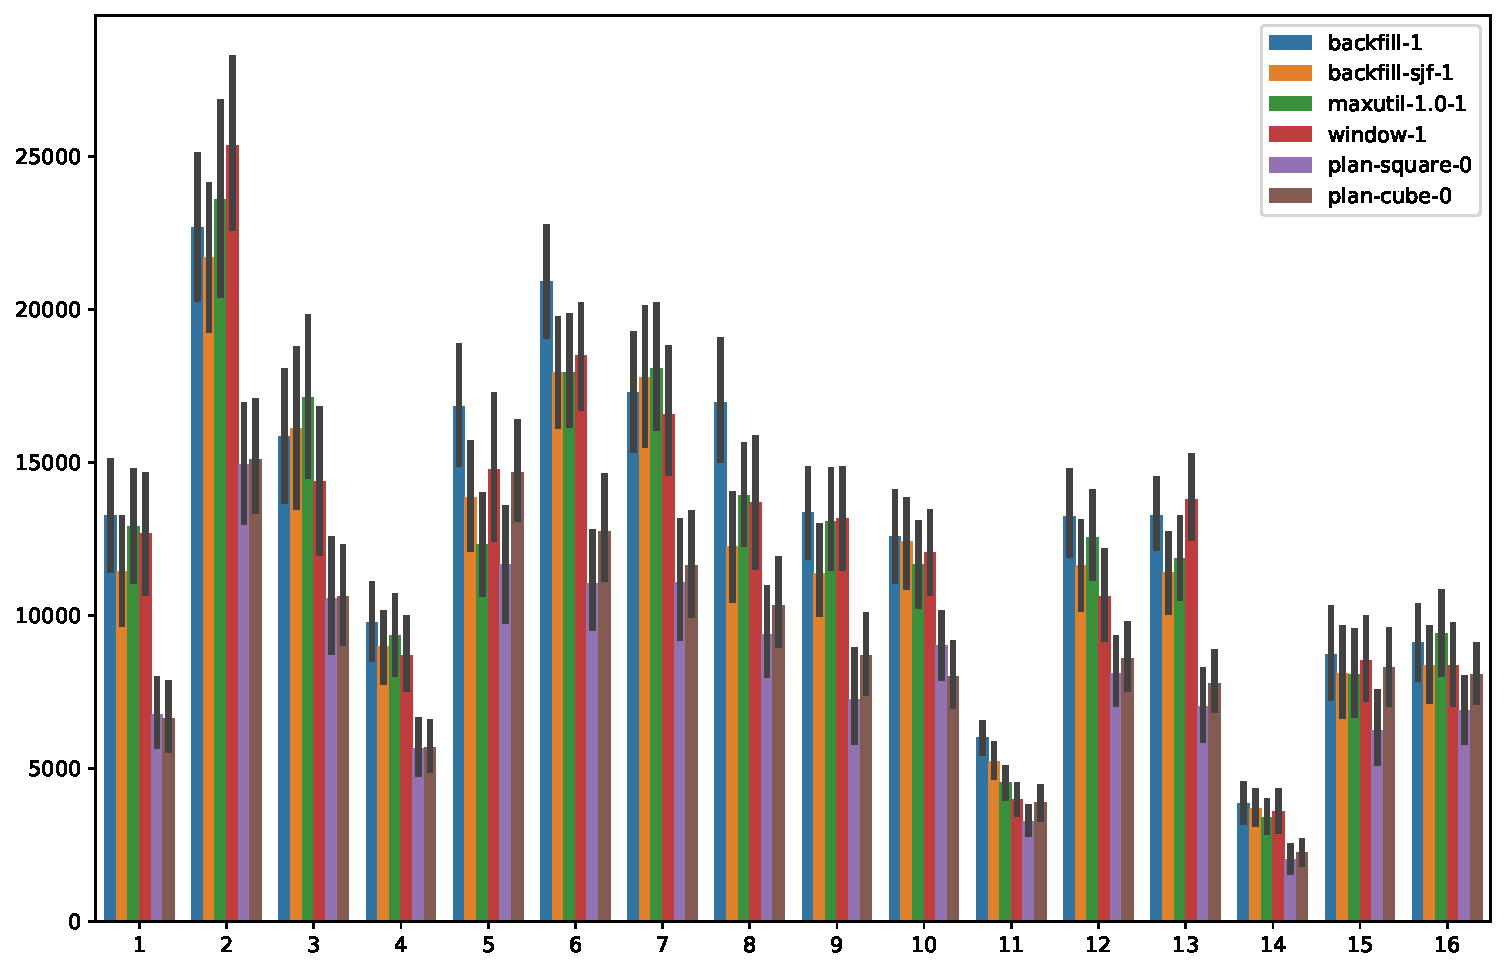
\includegraphics[width=\textwidth]{best_alloc-only_parts_waiting-time.pdf}
    \caption{Mean waiting time of the split workload}
    \label{fig:best_alloc-only_parts_waiting-time}
\end{figure}

\begin{figure}[p]
    \centering
    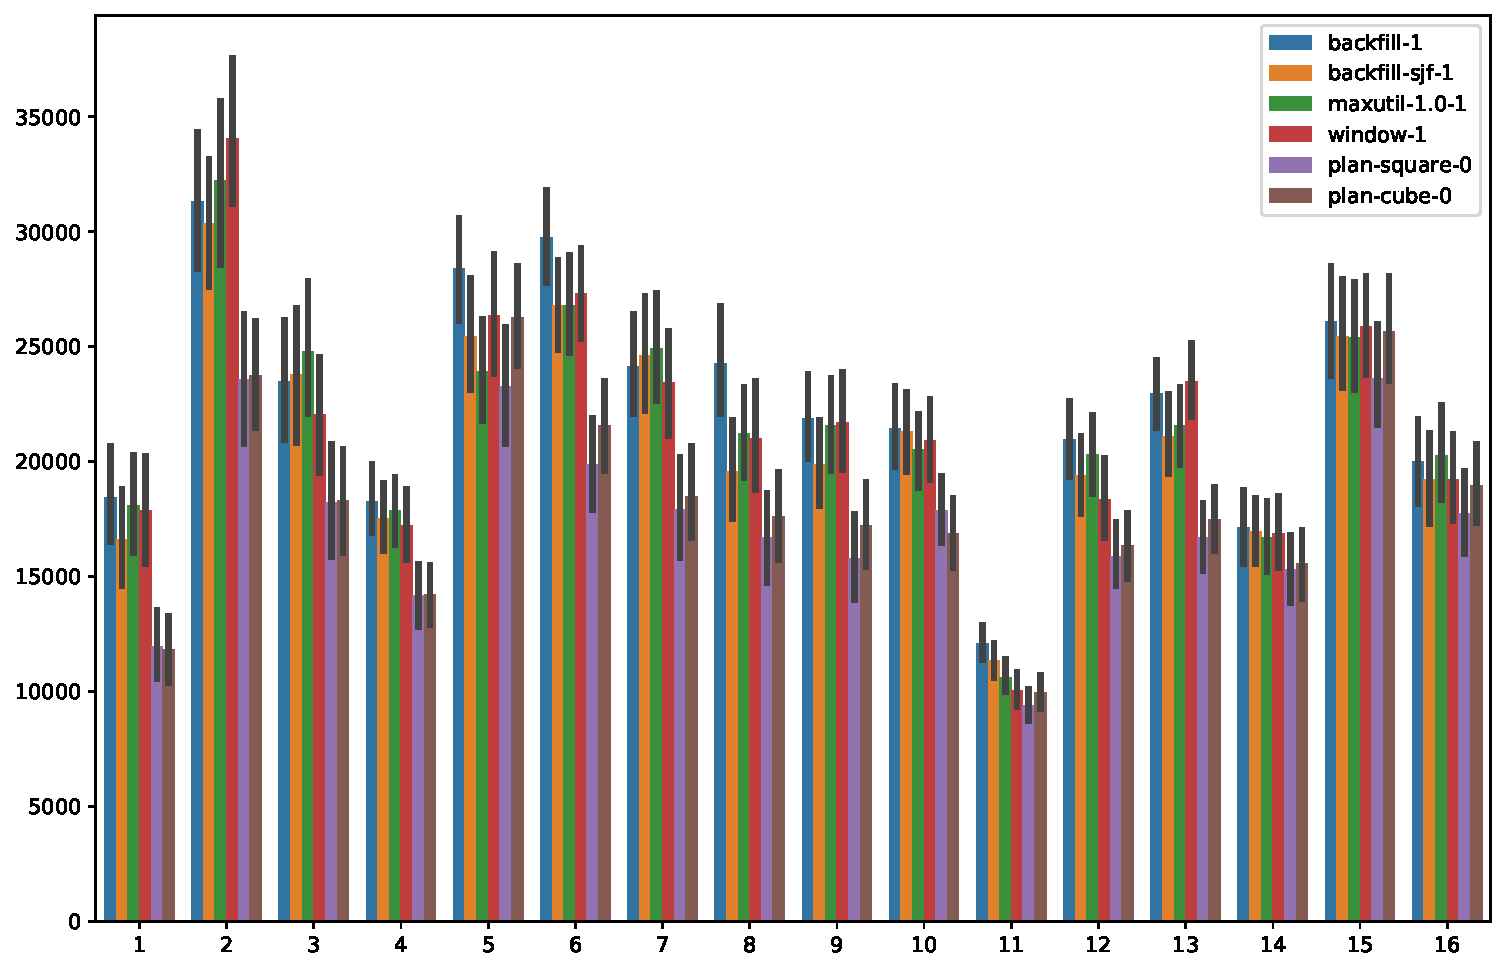
\includegraphics[width=\textwidth]{best_alloc-only_parts_turnaround-time.pdf}
    \caption{Mean turnaround time of the split workload}
    \label{fig:best_alloc-only_parts_turnaround-time}
\end{figure}

\begin{figure}[p]
    \centering
    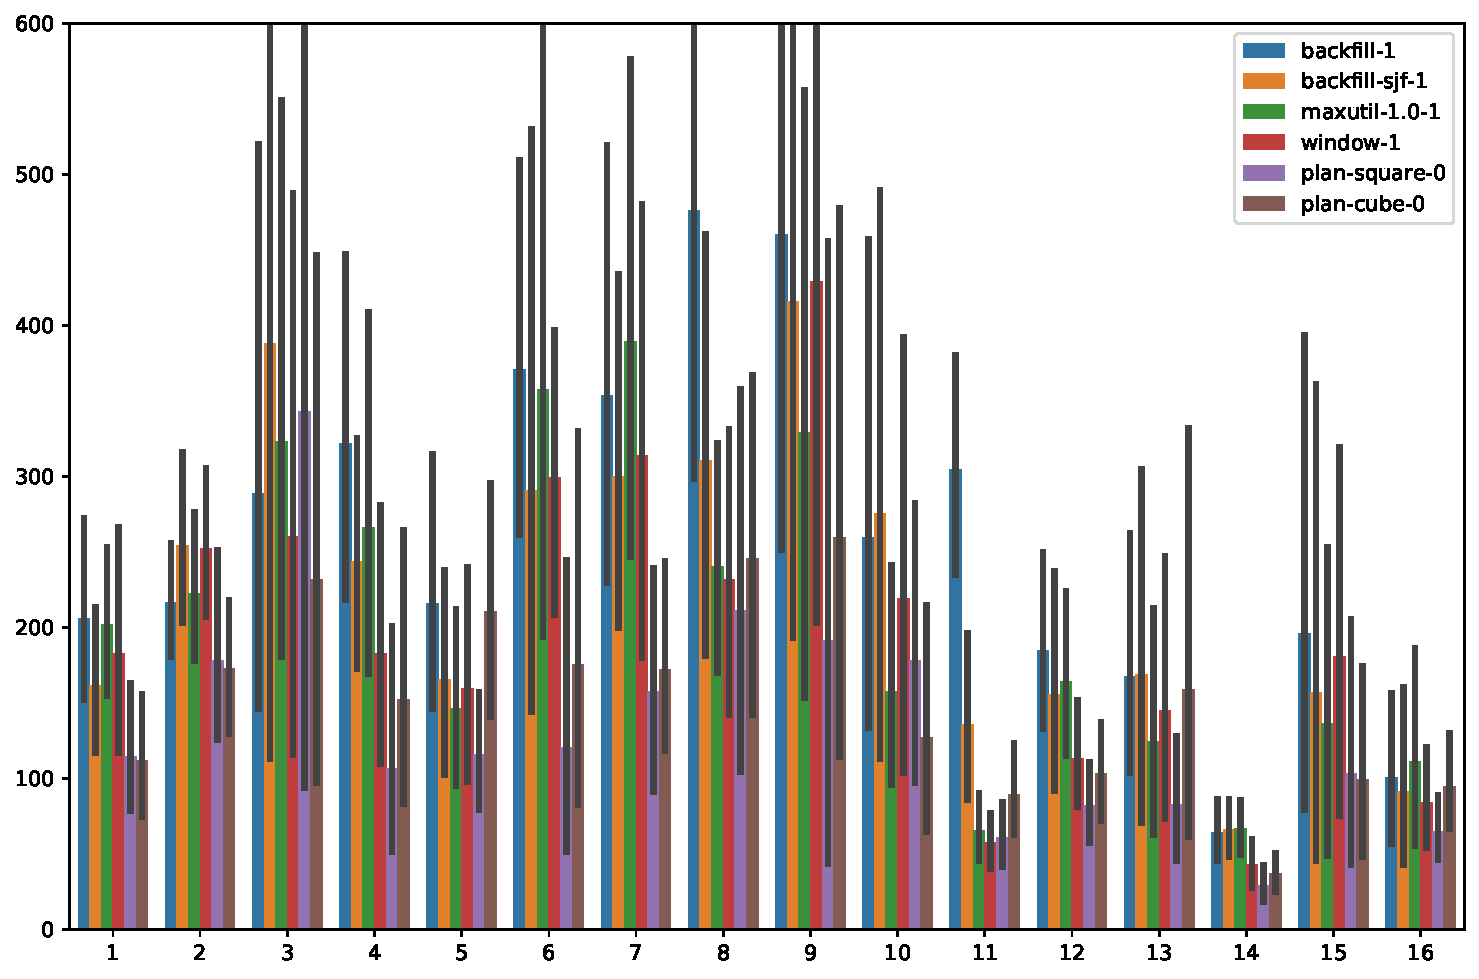
\includegraphics[width=\textwidth]{best_alloc-only_parts_slowdown.pdf}
    \caption{Mean slowdown of the split workload}
    \label{fig:best_alloc-only_parts_slowdown}
\end{figure}

\begin{figure}[p]
    \centering
    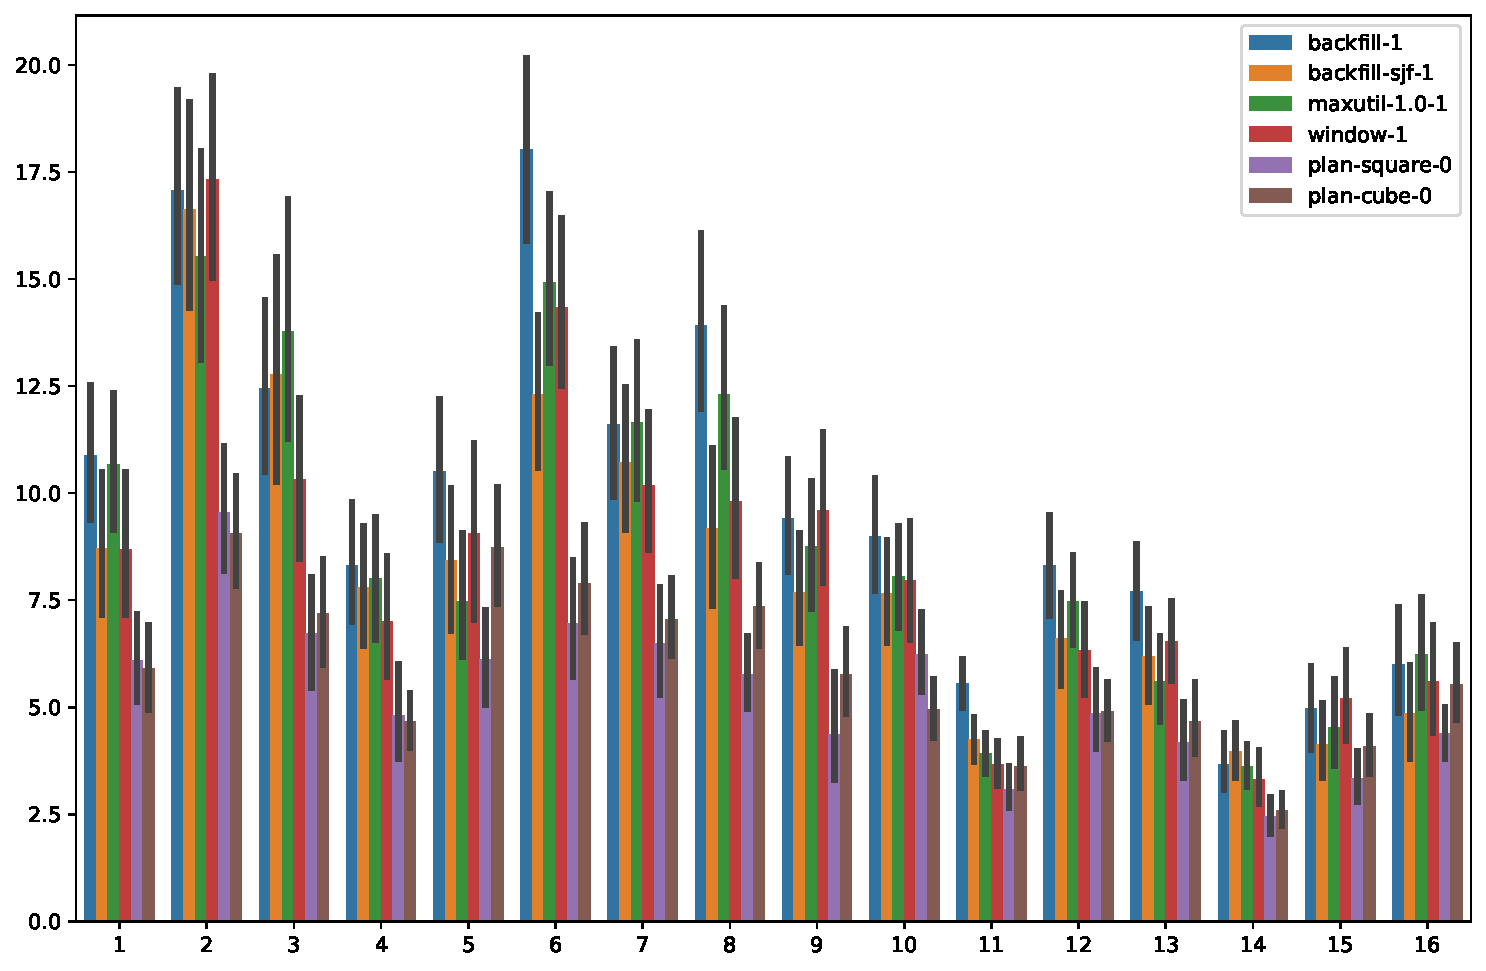
\includegraphics[width=\textwidth]{best_alloc-only_parts_bounded-slowdown.pdf}
    \caption{Mean bounded slowdown of the split workload}
    \label{fig:best_alloc-only_parts_bounded-slowdown}
\end{figure}

\begin{figure}[p]
    \centering
    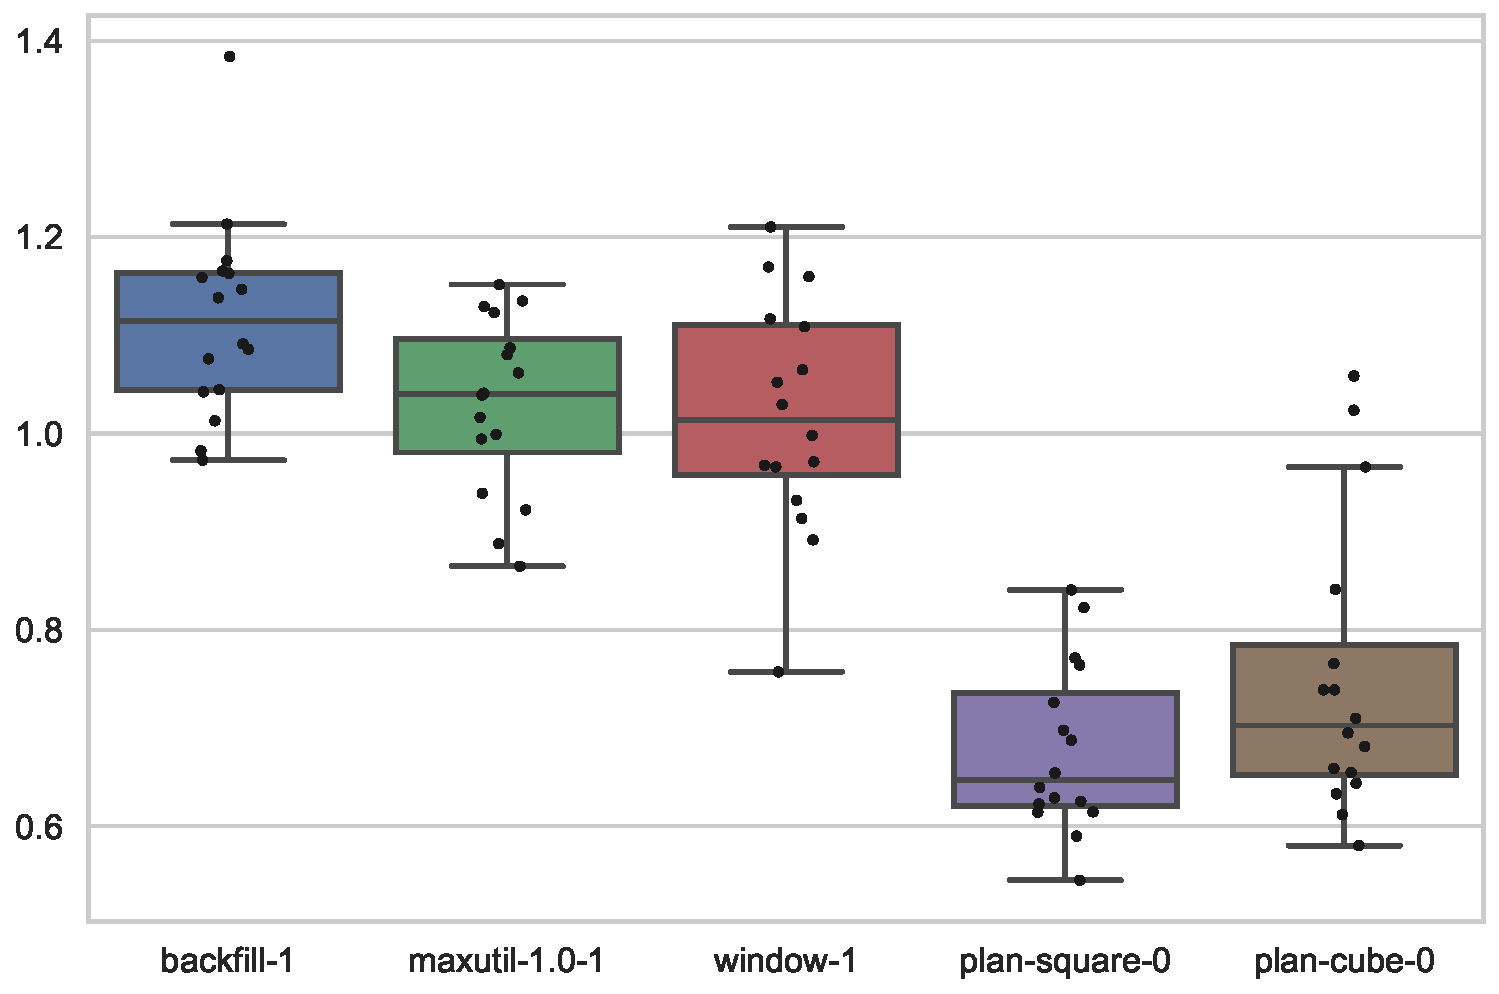
\includegraphics[width=\textwidth]{best_alloc-only_parts_waiting-time_box.pdf}
    \caption{Mean waiting time for each part in the split workload (normalised to backfill-sjf-1)}
    \label{fig:best_alloc-only_parts_waiting-time_box}
\end{figure}

\begin{figure}[p]
    \centering
    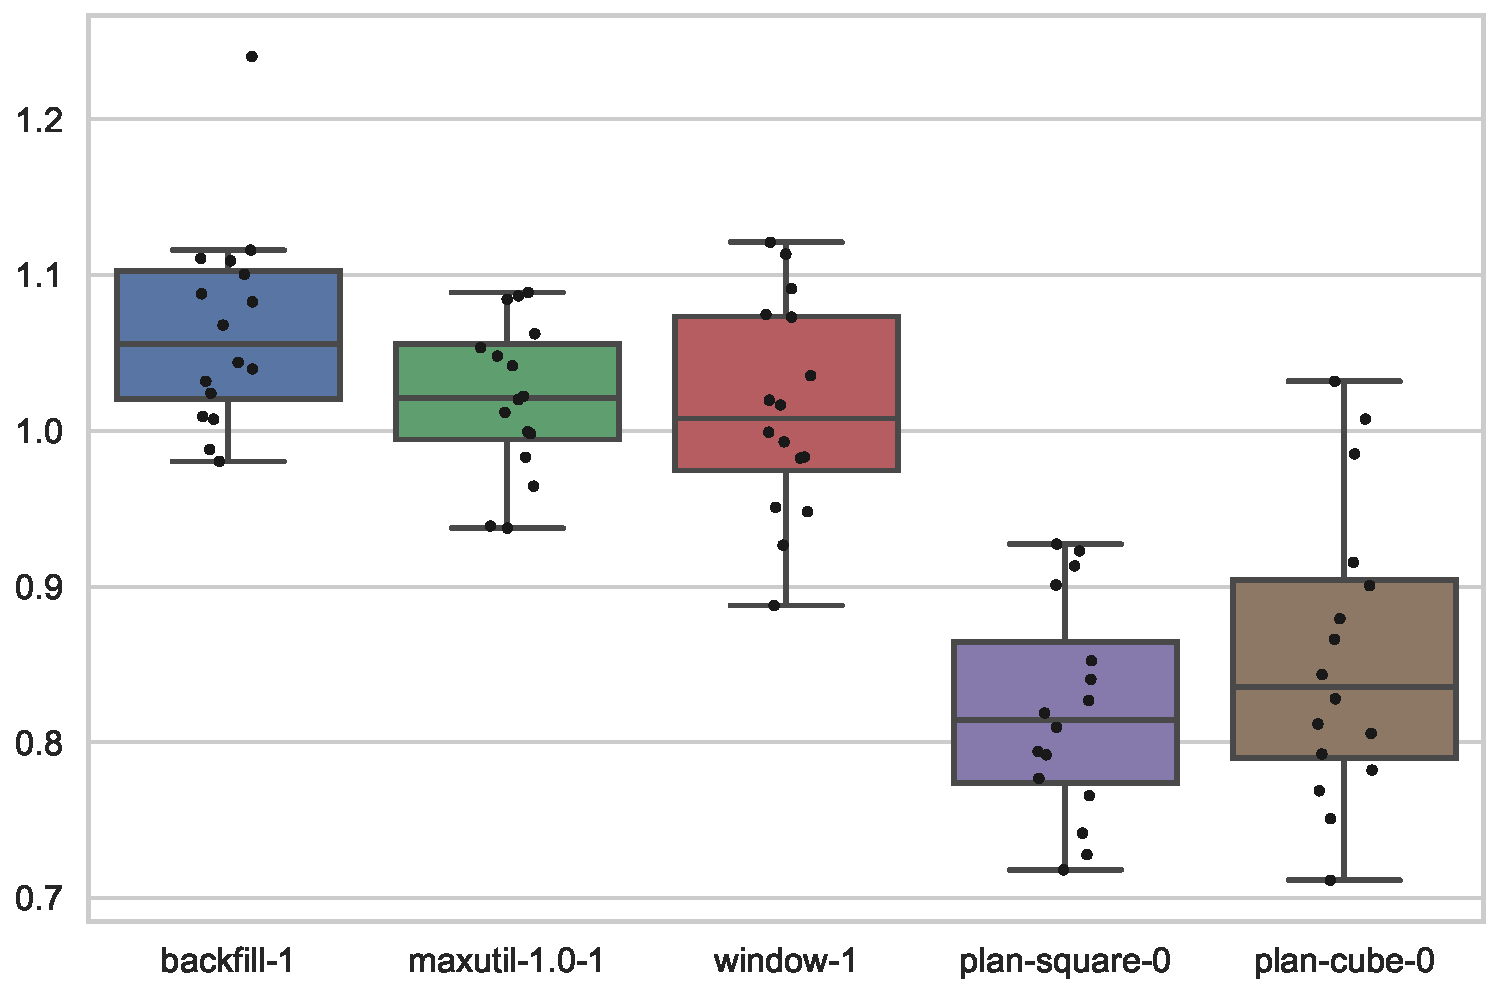
\includegraphics[width=\textwidth]{best_alloc-only_parts_turnaround-time_box.pdf}
    \caption{Mean turnaround time for each part in the split workload (normalised to backfill-sjf-1)}
    \label{fig:best_alloc-only_parts_turnaround-time_box}
\end{figure}

\begin{figure}[p]
    \centering
    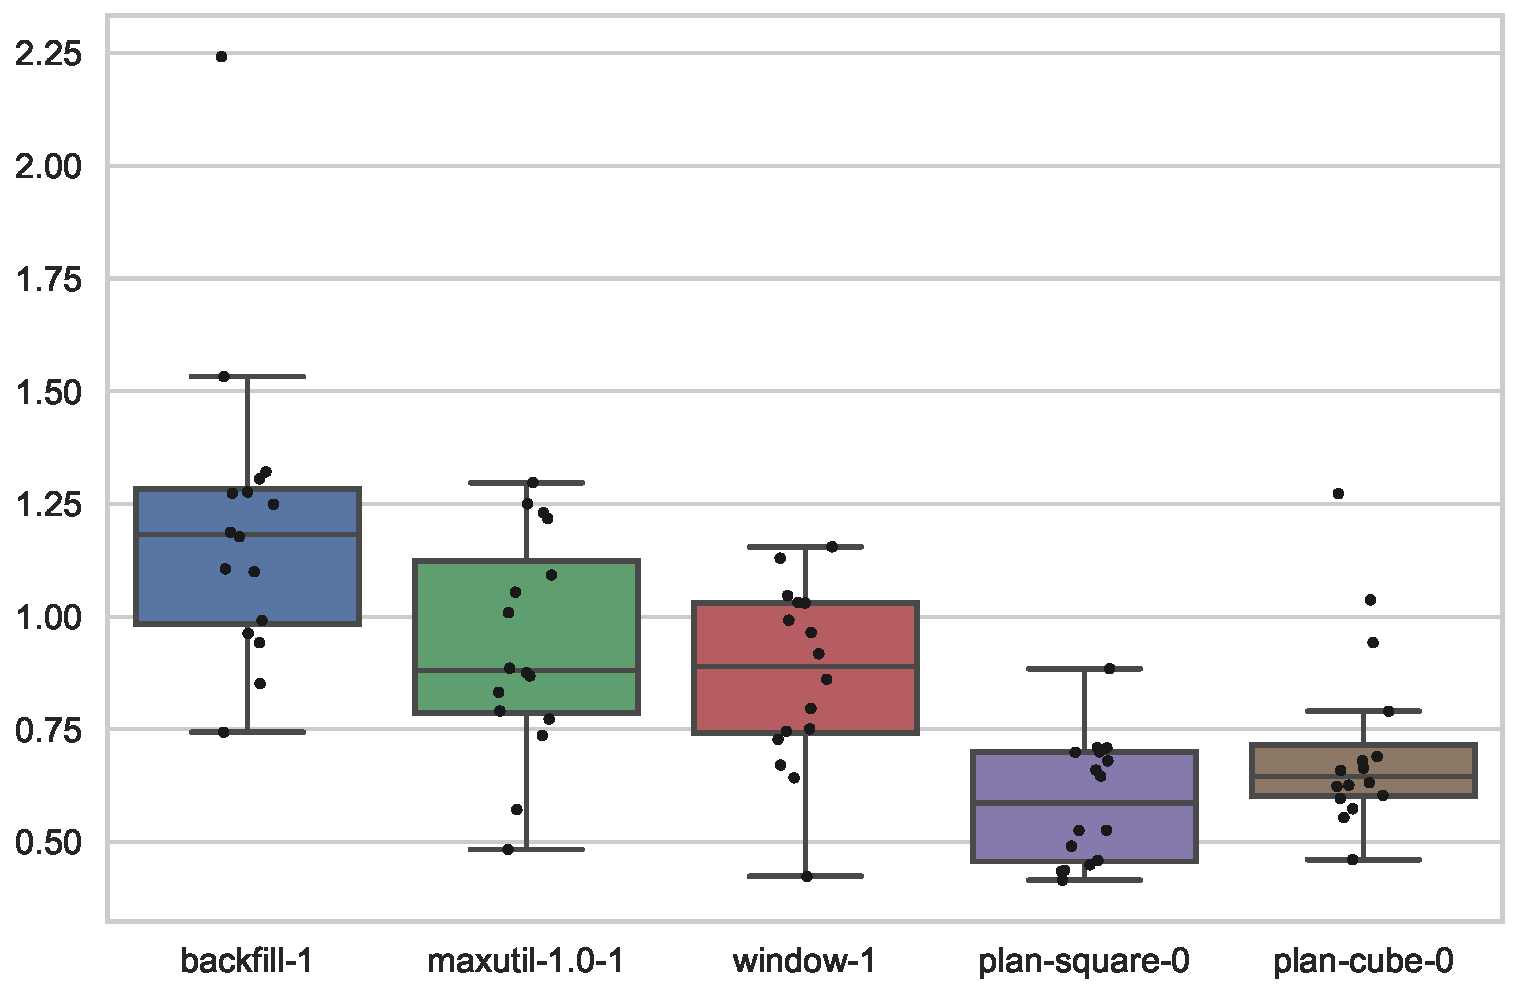
\includegraphics[width=\textwidth]{best_alloc-only_parts_slowdown_box.pdf}
    \caption{Mean slowdown for each part in the split workload (normalised to backfill-sjf-1)}
    \label{fig:best_alloc-only_parts_slowdown_box}
\end{figure}

\begin{figure}[p]
    \centering
    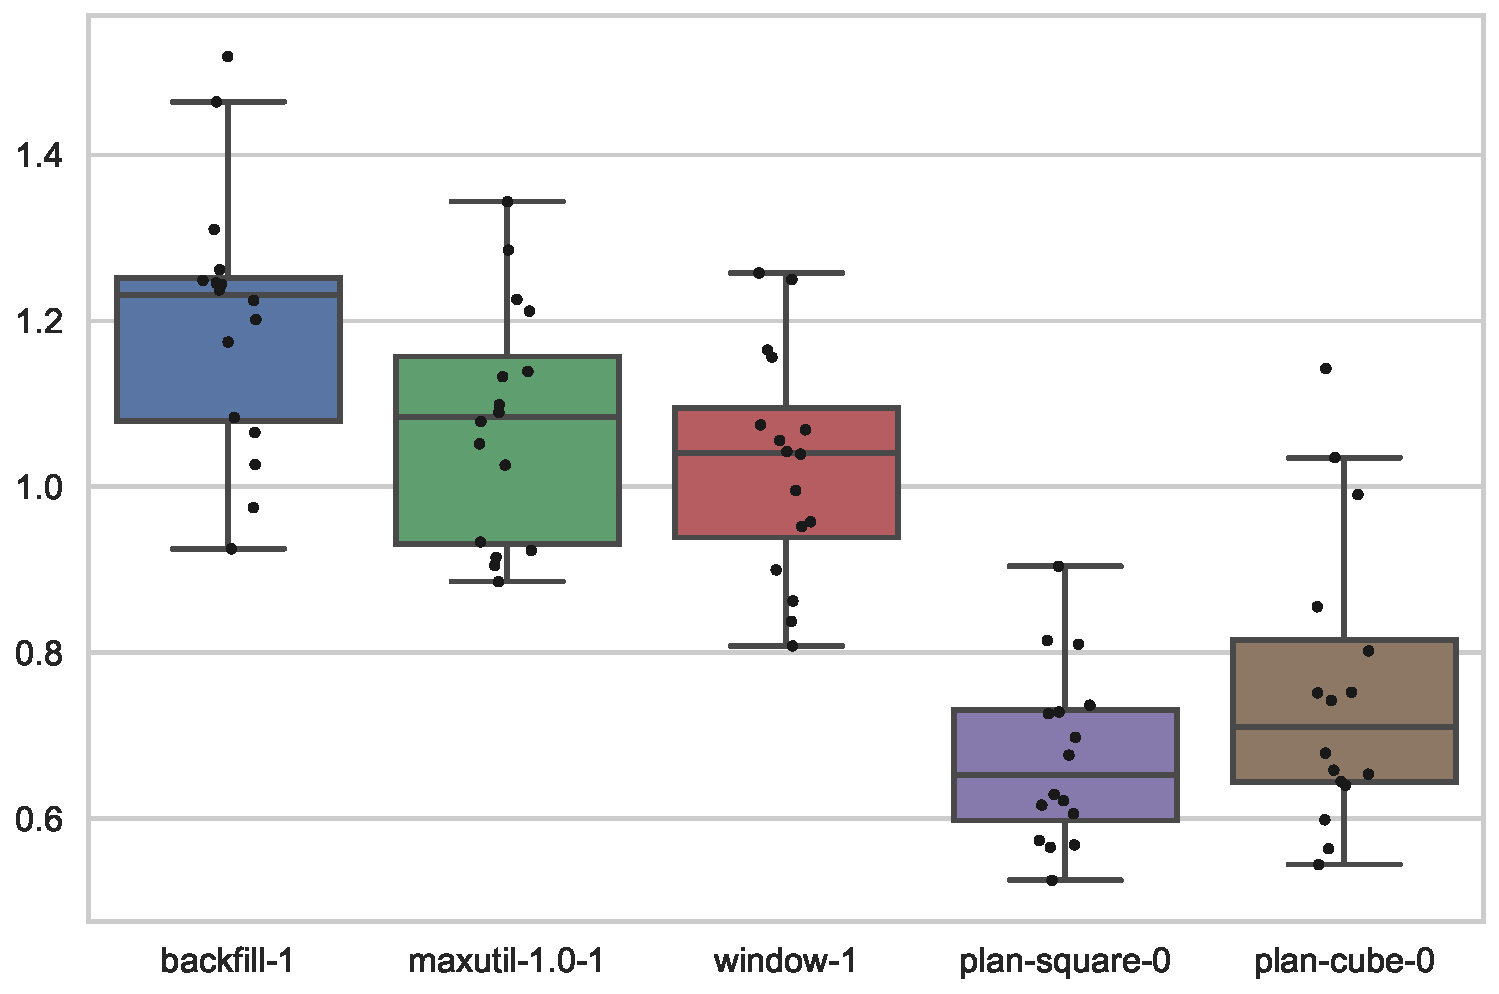
\includegraphics[width=\textwidth]{best_alloc-only_parts_bounded-slowdown_box.pdf}
    \caption{Mean bounded slowdown for each part in the split workload (normalised to backfill-sjf-1)}
    \label{fig:best_alloc-only_parts_bounded-slowdown_box}
\end{figure}

\FloatBarrier

\subsection{IO-Aware model}
\bestplot{io-aware}{waiting-time}{Waiting time}
\bestplot{io-aware}{turnaround-time}{Turnaround time}
\bestplot{io-aware}{slowdown}{Slowdown}
\bestplot{io-aware}{bounded-slowdown}{Bounded slowdown}

\begin{figure}[p]
    \centering
    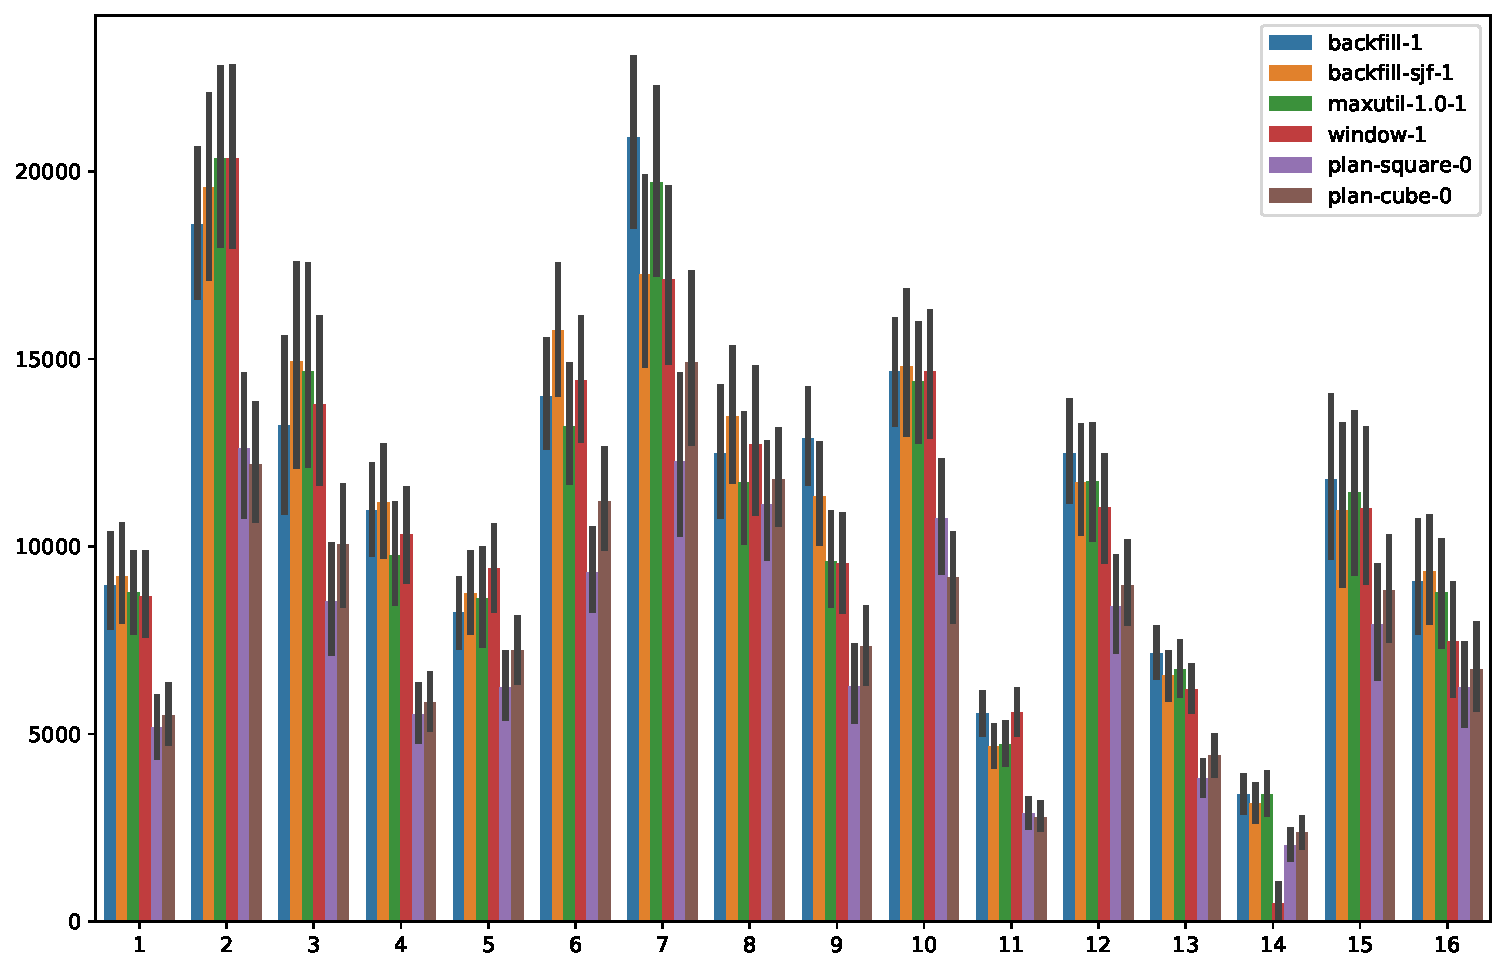
\includegraphics[width=\textwidth]{best_io-aware_parts_waiting-time.pdf}
    \caption{Mean waiting time of the split workload}
    \label{fig:best_io-aware_parts_waiting-time}
\end{figure}

\begin{figure}[p]
    \centering
    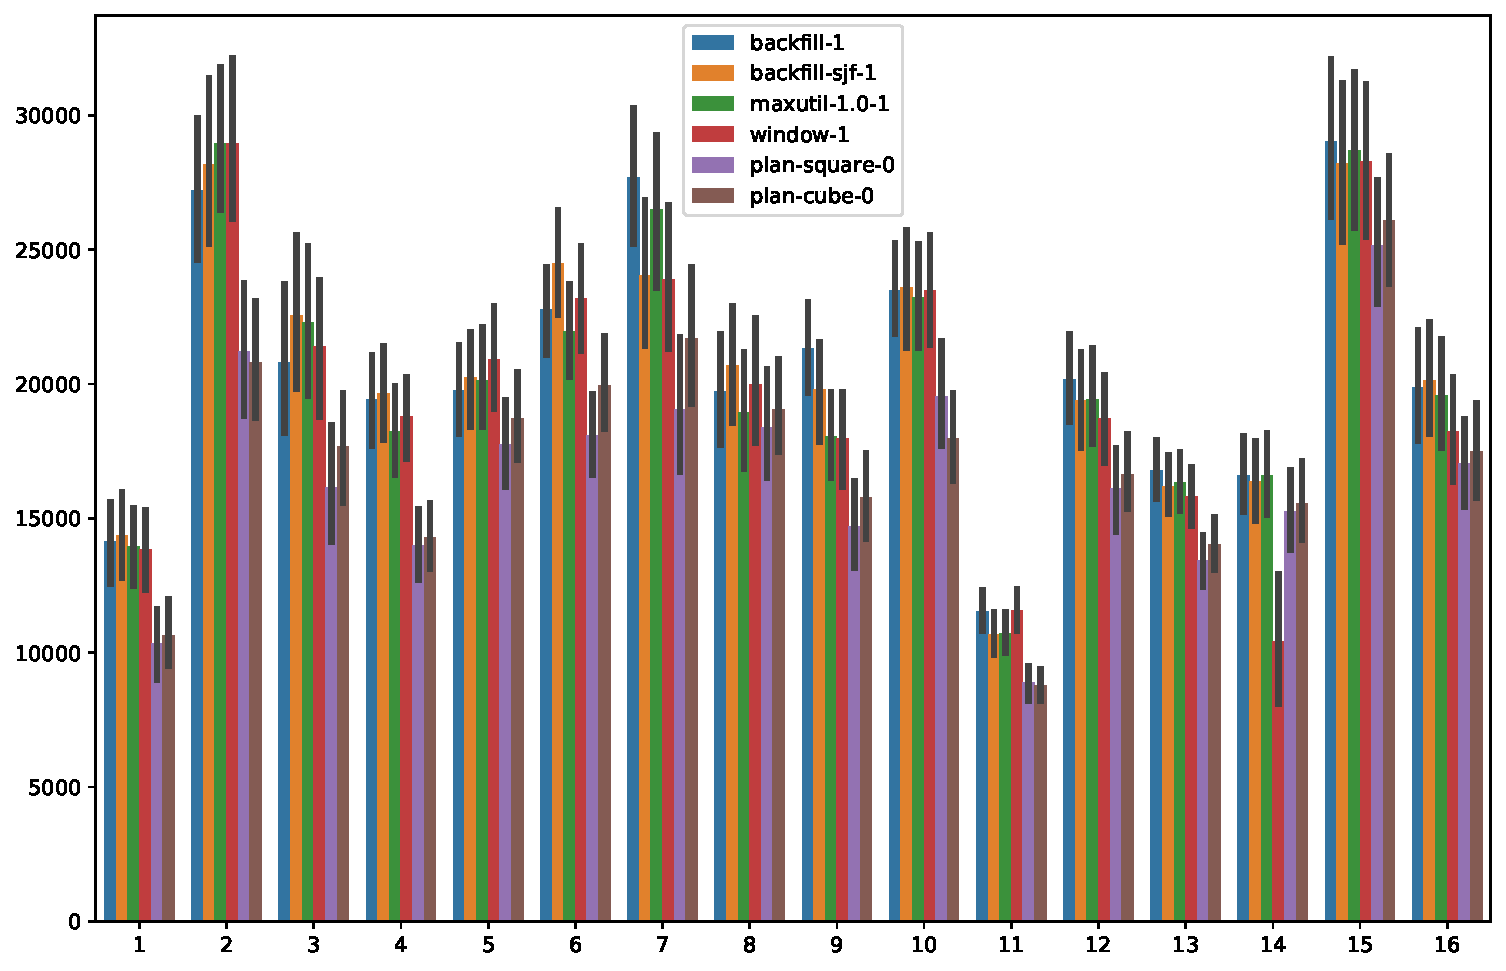
\includegraphics[width=\textwidth]{best_io-aware_parts_turnaround-time.pdf}
    \caption{Mean turnaround time of the split workload}
    \label{fig:best_io-aware_parts_turnaround-time}
\end{figure}

\begin{figure}[p]
    \centering
    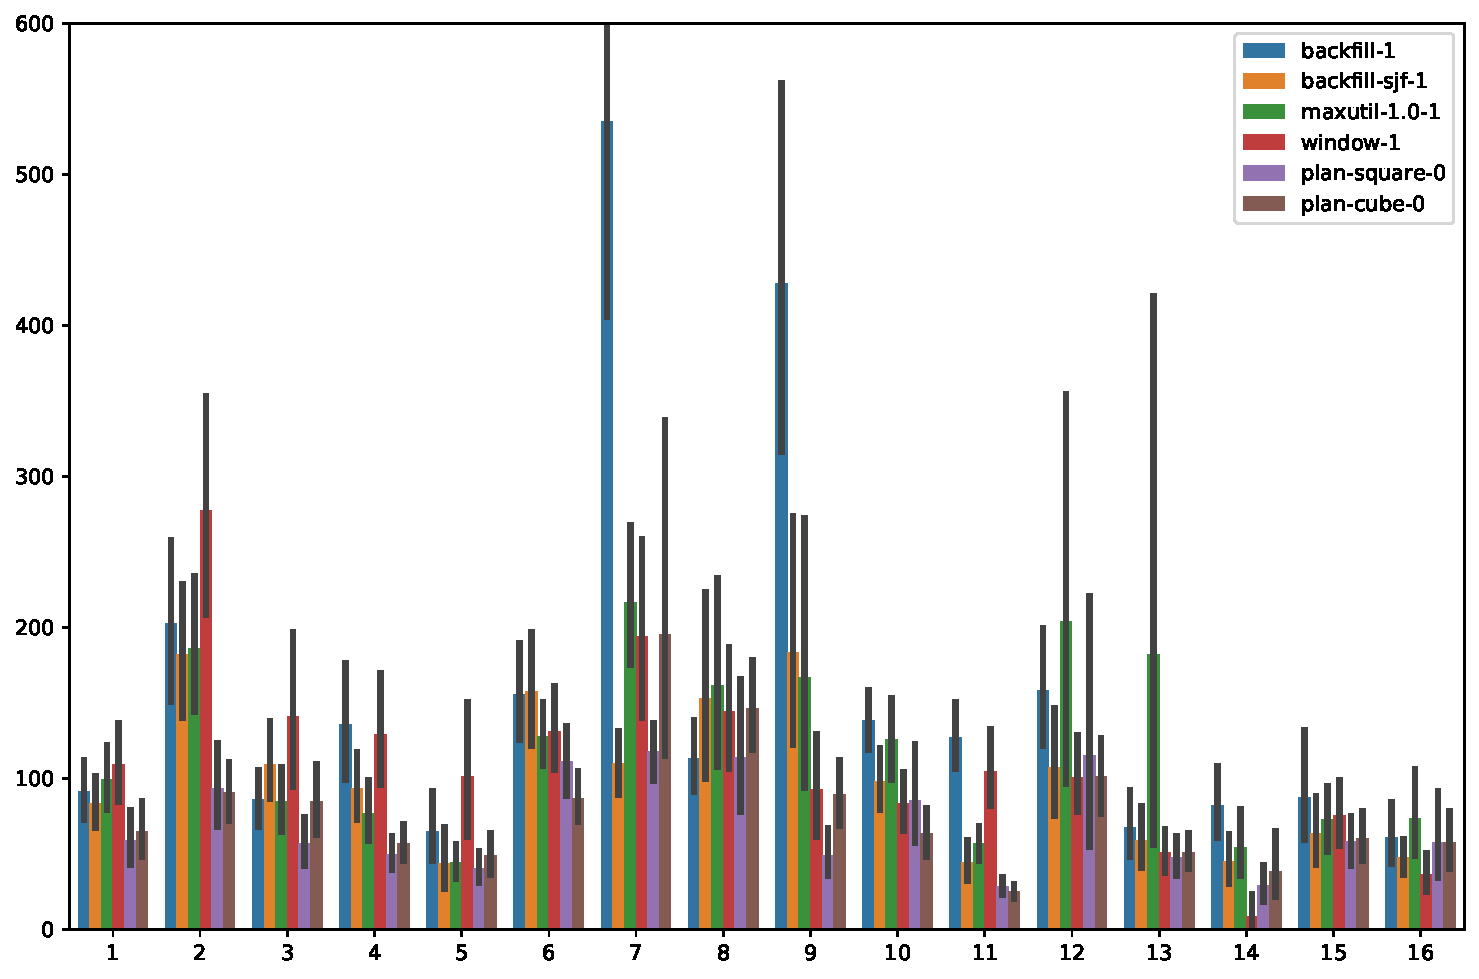
\includegraphics[width=\textwidth]{best_io-aware_parts_slowdown.pdf}
    \caption{Mean slowdown of the split workload}
    \label{fig:best_io-aware_parts_slowdown}
\end{figure}

\begin{figure}[p]
    \centering
    \includegraphics[width=\textwidth]{best_io-aware_parts_bounded-slowdown.pdf}
    \caption{Mean bounded slowdown of the split workload}
    \label{fig:best_io-aware_parts_bounded-slowdown}
\end{figure}

\begin{figure}[p]
    \centering
    \includegraphics[width=\textwidth]{best_io-aware_parts_waiting-time_box.pdf}
    \caption{Mean waiting time for each part in the split workload (normalised to backfill-sjf-1)}
    \label{fig:best_io-aware_parts_waiting-time_box}
\end{figure}

\begin{figure}[p]
    \centering
    \includegraphics[width=\textwidth]{best_io-aware_parts_turnaround-time_box.pdf}
    \caption{Mean turnaround time for each part in the split workload (normalised to backfill-sjf-1)}
    \label{fig:best_io-aware_parts_turnaround-time_box}
\end{figure}

\begin{figure}[p]
    \centering
    \includegraphics[width=\textwidth]{best_io-aware_parts_slowdown_box.pdf}
    \caption{Mean slowdown for each part in the split workload (normalised to backfill-sjf-1)}
    \label{fig:best_io-aware_parts_slowdown_box}
\end{figure}

\begin{figure}[p]
    \centering
    \includegraphics[width=\textwidth]{best_io-aware_parts_bounded-slowdown_box.pdf}
    \caption{Mean bounded slowdown for each part in the split workload (normalised to backfill-sjf-1)}
    \label{fig:best_io-aware_parts_bounded-slowdown_box}
\end{figure}

\FloatBarrier

\section{Backfilling reservation depth} \label{sec:depth}
In this section, we study the influence of the \emph{reservation depth} parameter ($D$) on selected scheduling algorithms. We want to find whether increasing the number of jobs taken to reservations from the front of the waiting queue improves or worsen the efficiency of scheduling. Moreover, we want to find an optimal value of the \emph{reservation depth} for each algorithm. We chose the canonical scheduling algorithms and the best performing plan-based policy. Namely, the selected algorithms are:
\begin{itemize}
    \item Greedy FCFS filling without any reservations (filler, Algorithm \ref{alg:filler})
    \item FCFS-backfilling with $D=1$ (backfill-1, Algorithm \ref{alg:backfill})
    \item FCFS-backfilling with $D=2$ (backfill-2, Algorithm \ref{alg:backfill})
    \item FCFS-backfilling with $D=3$ (backfill-3, Algorithm \ref{alg:backfill})
    \item FCFS-backfilling with $D=4$ (backfill-4, Algorithm \ref{alg:backfill})
    \item Greedy SJF filling without any reservations (filler-sjf)
    \item SJF-backfilling with $D=1$ (backfill-sjf-1, Algorithm \ref{alg:backfill-sjf})
    \item SJF-backfilling with $D=2$ (backfill-sjf-2, Algorithm \ref{alg:backfill-sjf})
    \item SJF-backfilling with $D=3$ (backfill-sjf-3, Algorithm \ref{alg:backfill-sjf})
    \item SJF-backfilling with $D=4$ (backfill-sjf-4, Algorithm \ref{alg:backfill-sjf})
    \item Plan-based minimising the sum of squared waiting time with $D=0$ (plan-square-0, $\alpha=2$, Algorithm \ref{alg:plan})
    \item Plan-based minimising the sum of squared waiting time with $D=1$ (plan-square-1, $\alpha=2$, Algorithm \ref{alg:plan})
    \item Plan-based minimising the sum of squared waiting time with $D=2$ (plan-square-2, $\alpha=2$, Algorithm \ref{alg:plan})
    \item Plan-based minimising the sum of squared waiting time with $D=3$ (plan-square-3, $\alpha=2$, Algorithm \ref{alg:plan})
\end{itemize}
Filler may be perceived as the FCFS-backfilling with $D=0$. Analogously, filler-sjf can be viewed as SJF-backfilling with $D=0$. We do not present plan-based scheduling with $D=4$ due to its extraordinary extensive computation time. We evaluate the algorithms only the IO-Aware model.

For all presented metrics, we see that increasing the \emph{reservation depth} above 1 deteriorate the scheduling performance for all algorithms. For FCFS and SJF backfilling, the results of the mean and all ordered statistics are monotonically increasing. The variants of those scheduling algorithms without reservations, filler and filler-sjf, also shows worse results than backfilling with $D=1$. 

For the plan-based policy, all results are monotonically increasing in terms of the mean values and quantiles.

The tail distributions plots indicate interesting results as well. At first, we want to point out that the tail distribution plots for waiting time, turnaround time and bounded slowdown were truncated. Specifically, for some jobs, filler-sjf resulted in values even an order of magnitude higher than the worst scores for scheduling policies with $D=1$. Presenting all values for filler-sjf would dominate other algorithms and make them  indistinctive. In general filler and filler-sjf have significantly worse tail distributions that all other policies. Excluding greedy filling algorithms, the dispersion of tail distributions is increasing with the $D$ parameter.

Based on our experiments for the full workload in the IO-Aware model, we conclude that the optimal \emph{reservation depth} for canonical FCFS and SJF backfilling is 1. Whereas, for plan-based scheduling, which is minimising the sum of squared waiting time, no reservations results with the best outcome.

\depthplot{waiting-time}{Waiting time}
\depthplot{turnaround-time}{Turnaround time}
\depthplot{slowdown}{Slowdown}
\depthplot{bounded-slowdown}{Bounded slowdown}
\end{document}